\documentclass[preprint,review,12pt]{elsarticle}

\pdfoutput=1
%% Use the options 1p,twocolumn; 3p; 3p,twocolumn; 5p; or 5p,twocolumn
%% for a journal layout:
%% \documentclass[final,1p,times]{elsarticle}
%% \documentclass[final,1p,times,twocolumn]{elsarticle}
%% \documentclass[final,3p,times]{elsarticle}
%% \documentclass[final,3p,times,twocolumn]{elsarticle}
%% \documentclass[final,5p,times]{elsarticle}
%% \documentclass[final,5p,times,twocolumn]{elsarticle}

%% For including figures, graphicx.sty has been loaded in
%% elsarticle.cls. If you prefer to use the old commands
%% please give \usepackage{epsfig}

\usepackage{amssymb}
\usepackage{tikz}

%\usepackage[utf8]{inputenc}
\usepackage[greek, british]{babel}
\usepackage{alphabeta}
\usepackage{libertine}
\usepackage{csquotes}
\usepackage{hyperref}
\usepackage{float}
\usepackage{amsmath}
\graphicspath{ {./images/} }
\usepackage[a4paper,margin=1in,footskip=0.25in]{geometry}
\usepackage{etoolbox}
\makeatletter
\def\ps@pprintTitle{%
    \let\@oddhead\@empty
    \let\@evenhead\@empty
    \def\@oddfoot{\footnotesize\itshape
         {Submitted preprint} \hfill\today}%
    \let\@evenfoot\@oddfoot
    }
\makeatother

\newcommand{\xmark}{%
\tikz[scale=0.23] {
    \draw[line width=0.7,line cap=round] (0,0) to [bend left=6] (1,1);
    \draw[line width=0.7,line cap=round] (0.2,0.95) to [bend right=3] (0.8,0.05);
}}




\setcounter{secnumdepth}{4}
\setcounter{tocdepth}{4}

\pagenumbering{arabic}
%% The lineno packages adds line numbers. Start line numbering with
%% \begin{linenumbers}, end it with \end{linenumbers}. Or switch it on
%% for the whole article with \linenumbers.
%% \usepackage{lineno}

%\journal{Information Sciences}

\begin{document}

\begin{frontmatter}

\title{Neural Natural Language Processing for Long Texts: A Survey of the State-of-the-Art}

\author{Dimitrios Tsirmpas$\dagger$, Ioannis Gkionis$\dagger$, Ioannis Mademlis*}
\address{Department of Informatics, Athens University of Economics and Business}
\fntext[myfootnote1]{$\dagger$ The first two authors contributed equally and are joint first authors.}
\fntext[myfootnote2]{*Ioannis Mademlis is the corresponding author.}
% \author[first]{Dimitrios Tsirmpas\dagger}\ead{tsirbasdim@gmail.com}
% \author[second]{Ioannis Gkionis\dagger}\ead{yannisgionis1@gmail.com}\footnote{\dagger denotes joint first authorship and equal contribution.}
% \author[cor]{Ioannis Mademlis\corref{cor}} \ead{imademlis@aueb.gr} 
% \cortext[cor]{corresponding author}
% \affiliation[first,second,cor]{organization={Department of Informatics, Athens University of Economics and Business},
%             addressline={Patision 76}, 
%             city={Athens},
%             postcode={GR-10434},
%             country={Greece}}
            
\begin{abstract}
The adoption of Deep Neural Networks (DNNs) has greatly benefited Natural Language Processing (NLP) during the past decade. However, the demands of long documents analysis are quite different from those of shorter texts, with the ever increasing size of documents uploaded online rendering NLP on long documents a critical area of research. This paper surveys the current state-of-the-art in the domain, overviewing the relevant neural building blocks and subsequently focusing on two main NLP tasks: Document Classification, Summarization as well as mentioning uses in Sentiment Analysis. We detail the challenges, issues and current solutions related to long-document NLP. We also list publicly available, labelled, long-document datasets used in current research.
\end{abstract}

%%Graphical abstract
%\begin{graphicalabstract}
%\includegraphics{grabs}
%\end{graphicalabstract}

%%Research highlights
% \begin{highlights}
% \item Research highlight 1
% \item Research highlight 2
% \end{highlights}

\begin{keyword}
Natural Language Processing \sep long document \sep Document Classification \sep Document Summarization \sep Sentiment Analysis \sep opinion mining \sep Deep Neural Networks
\end{keyword}

\end{frontmatter}


\section{Introduction}
Understanding written text has always been an area of significant interest not only for Artificial Intelligence (AI) research but also for increasingly many commercial applications. Successfully parsing and analyzing text expressed in natural language is crucial for a variety of tasks traditionally performed by humans, which require the extraction of sentiments, meaning or themes. Books \cite{worsham}, academic papers \cite{gales}, technical manuals \cite{nabizadeh}, news articles \cite{shuo}, legal documents \cite{merchant} and many other types of long texts can be the target of such tasks.

Natural Language Processing (NLP) is the field of AI dedicated to developing algorithms for the semantic understanding of written and spoken language. NLP methods can be differentiated by the level of granularity they operate on. \textit{Sentence-level} NLP examines individual sentences and their structure, grammar, and meaning. This type of analysis is useful for tasks such as Sentiment Analysis or named entity recognition, which can be performed on a sentence-by-sentence basis \cite{borgir}. \textit{Paragraph-level} NLP analysis involves examining the larger context in which sentences are used. This type of analysis can help identify the topic or theme of a paragraph, as well as the relationships between sentences within the paragraph and is usually used as an intermediate stage between sentence-level and document-level analysis \cite{andrew} \cite{guo} \cite{jiwei}. \textit{Document-level} NLP analysis involves analyzing an entire document, such as a book, article, or email. This type of analysis can provide insights into the overall content, sentiment, and style of the document \cite{wei}\cite{timothy}. Document-level analysis can also involve tasks such as Document Classification or summarization, which require understanding the content of the document as a whole. This paper focuses exclusively on document-level analysis, or long-document NLP, for documents that are longer than just a few paragraphs.

Similarly to the more common case of short text analysis, long-document NLP has been revolutionized during the past decade by Deep Neural Networks (DNNs), which greatly surpassed traditional statistical and machine learning approaches in accuracy and abilities. Nevertheless, even DNNs face severe challenges when analyzing very long documents, due to a higher chance of ambiguities, varying context, potentially lower coherence, etc. \cite{hold}. Despite such limitations though, long-document NLP has already become very important in the industry. For example, a recent study \cite{vithya} demonstrates how NLP can be used to extract medical categories from electronic health records, enabling better patient care and treatment plans. Other recent methods \cite{lulu} \cite{bambroo} utilize DNNs to automatically classify lengthy legal documents. In fact, the legal domain is currently one of the major application areas of long-document NLP, with relevant algorithms exploited for desk research, electronic discovery, contract review, document automation, and even legal advice \cite{dale}.

This survey focuses on two key NLP tasks that present peculiarities for the long-document case: \textit{Document Classification} and \textit{Document Summarization}, The first involves categorizing entire documents into predefined classes, based on their content. This enables efficient organization and retrieval of information. The second aims to generate concise and coherent summaries of longer documents. It involves distilling the key information and main ideas from a document, while preserving its meaning.

Additionally, \textit{Sentiment Analysis} is also investigated as a particular variant of Document Classification. The task consists in determining the sentiment or emotional tone expressed in a piece of text, such as positive, negative, or neutral. It involves analyzing subjective opinions, attitudes, and emotions expressed in reviews, social media posts, or customer feedback.

Before the rise of DNNs, traditional machine learning methods were typically used for executing NLP tasks. For instance, Latent Dirichlet Allocation (LDA) \cite{dirichet} is a popular unsupervised learning method that categorizes documents into $k$ topics, according to their \textit{tokens}. Tokens in this case would be individual words, but for other algorithms may be sentences, expressions, or subwords \cite{tokens}. The concept of tokens serves as a building block in defining more complex textual structures, such as \textit{n-grams} \cite{ngrams}. These are continuous sequences of $n$ tokens, which can be exploited by NLP algorithms to capture the context and/or the sequential dependencies within text. For a comprehensive coverage of relevant traditional approaches, the reader is referred to \citet{korde}.

Despite the presence of review papers discussing the development, methodology and applications of NLP tasks in general \cite{kowasari} \cite{torfi} \cite{chai}, or in specific thematic fields \cite{nielker} \cite{qian} \cite{gupta} \cite{hussein}, there are currently to our knowledge no survey/review articles discussing and aggregating recent research on long-document NLP using DNNs. To remedy such gaps in existing literature, this article specifically focuses on long-document NLP. It overviews the relevant neural building blocks and systematically reviews existing solutions to three main NLP tasks for long documents (Classification, Summarization, Sentiment Analysis). It then identifies current challenges, discussing how they impact long-document NLP and presents existing ways to circumvent them. The goal of this article is two-fold: i) to make the barrier of entry for this relatively very young section of active research more accessible to the community, and ii) to aggregate common issues and solutions in various common NLP tasks, in the domain of long-document analysis.

The remainder of this article is organized in the following manner. Section \ref{sec::existingReviews} details previous recent surveys/reviews that overlap with this article, highlighting the main differences. Section \ref{sec::DNNs} briefly overviews basic to state-of-the-art neural architectures and building blocks for NLP. Sections \ref{sec::Classification}, \ref{sec::Summarization} and \ref{sec::Sentiment} detail the challenges and proposed solutions to the Document Classification, Summarization and Sentiment Analysis tasks respectively, focusing on long documents. Section \ref{sec::Datasets} presents publicly available, annotated long-document datasets, which can be utilized for relevant research. Section \ref{sec::Summary} summarizes and organizes the above methods and challenges, discusses current and future trends and identifies open issues. Finally, in Section \ref{sec::Conclusions} we follow up with our conclusions and discuss the current state and future of long-document NLP research.
    
\section{Relevant previous reviews}
\label{sec::existingReviews}

\begin{table}[H]
        \centering
         \begin{tabular}
             { |p{4cm}|p{1cm}|p{1cm}|p{1cm}|p{1cm}|p{1cm}|p{2cm}|}
             \hline
             \textbf{Review}&\cite{kowsari}&\cite{wagh}&\cite{koh}&\cite{omori}&\cite{poon}&This article\\
             \hline
             Document Classification&\checkmark&\checkmark&\xmark&\xmark&\xmark&\checkmark\\
             \hline
             Document Summarization&\xmark&\xmark&\checkmark&\xmark&\xmark&\checkmark\\
             \hline
             Sentiment Analysis&\xmark&\xmark&\xmark&\checkmark&\checkmark&\checkmark\\
             \hline
             Relevant Neural Networks&\checkmark&\checkmark&\xmark&\xmark&\checkmark&\checkmark\\
             \hline
             Long Texts&\xmark&\checkmark&\checkmark&\checkmark&\xmark&\checkmark\\
             \hline
             Issue Discussion&\xmark&\checkmark&\checkmark&\xmark&\xmark&\checkmark\\
             \hline
             Issue Aggregation&\xmark&\xmark&\xmark&\xmark&\xmark&\checkmark\\
             \hline
             long-document Datasets&\xmark&\xmark&\checkmark&\xmark&\xmark&\checkmark\\
             \hline
        \end{tabular}
    \caption{Comparisons between notable existing reviews and this article.}
    \label{tab::review_table}
\end{table}

The Document Classification task has been covered extensively by \citet{kowsari}, where the terminology, basic concepts, metrics, preprocessing strategies and current learning approaches are covered. In \citet{wagh}, this analysis is extended to long texts and traditional machine learning models are compared with modern DNNs. Document Summarization, by its very nature, is closely tied with the challenges of long documents. In \citet{koh}, a thorough survey of state-of-the-art models, datasets and metrics is offered. Sentiment Analysis (alternatively "Opinion Mining") typically concerns short documents, such as reviews, comments and social media posts. However, a review of modern approaches to a specific subtask of Sentiment Analysis is conducted in \citet{omori}, where the goal is to analyze entire literary works with respect to their story and emotions. More generally, \citet{poon} provides an overview of Sentiment Analysis algorithms and current DNN solutions.

While these reviews certainly overlap with this article, to our knowledge there is no previous effort for aggregating and comparing the issues and challenges posed by long documents across multiple NLP tasks, while focusing exclusively on modern DNNs. This articlethus  attempts to expose common issues and encourage researchers to either adopt novel solutions, or use tried-and-tested  solutions from other NLP tasks. Our article also includes a Section focusing exclusively on long-Document Classification, which seems to be absent from relevant literature so far.

A simplified comparison between the above mentioned reviews and this article can be found in Table \ref{tab::review_table}. The row ``Issue Discussion" indicates that the paper specifically discusses issues with long texts/documents, while the row ``Issue Aggregation" indicates that issues are aggregated and compared across different NLP tasks.

    
\section{Deep Neural Networks for long-document analysis}
\label{sec::DNNs}
NLP tasks place specific demands on DNNs: for instance, a DNN model needs to uncover on its own the structure, context and the meaning of a single word. This calls for specialized architectures whose properties allow the DNN to navigate through the complexities of human-generated natural text. Long documents exacerbate these challenges, since: i) the context, the tone and the theme may change repeatedly as the text progresses, and ii) the DNN may be required to correlate semantic cues which are far apart to each other within the text, in order to successfully execute the desired task.

Since the state-of-the-art in NLP has been revolving around DNNs for the last several years, this Section briefly presents the most widespread and effective neural architectures used for NLP. The complexities and the individual variations of each architecture are out of the scope of this article, since its focus is on DNN-enabled long-document NLP and not on DNNs themselves. All architectures presented in this Section are typically trained with variants of error back-propagation and stochastic gradient descent \cite{rumelhart} \cite{jordan}, but only the inference stage is described here.

The following presentation is split into two Subsections. Initially, generic neural architectures are briefly described for reference purposes (MLP, CNN, RNN/LSTM, Transformer). Subsequently, specific NLP-oriented neural architectures commonly used for analysing long texts are detailed.


\subsection{General Neural Architectures}

\subsubsection{MultiLayer Perceptrons}
The most common and traditional form of neural networks utilized for NLP is the well-known MultiLayer Perceptron (MLP). It is a relatively simple feed-forward architecture which consists of an input layer, one or more hidden layers and an output layer. An MLP with more than a few hidden layers typically qualifies as a deep architecture, although there is no precise threshold for discriminating strictly between shallow and deep models. Each hidden neuron acts as a postsynaptic neuron across different weighted synapses, separately connecting it with each of the neurons of the previous layer; thus, a main property of MLPs is that their layers are \textit{fully connected}. The scalar output of each neuron is transformed by an activation function, before being transmitted as input to the neurons of the next layer. The input layer typically receives as its input a fixed-size vector and, therefore, has as many neurons as the fixed and known dimensionality of the supported data points. Τhe majority of popular feed-forward neural architectures follow this basic concept at a coarse level and have essentially evolved from MLP. Notably, significant developments in neural network algorithms emerged gradually through attempts to solve the well-known \textit{vanishing gradient} problem: an issue of back-propagation-based training, which originally limited the realistically achievable number of hidden layers in MLPs (depth).

Eqs. (\ref{eq::MLP1})-(\ref{eq::MLP2})-(\ref{eq::MLP3}) below succinctly capture the inference-stage processing taking place in MLP. The output of one single neuron is given by:

\begin{equation}
    o = f(\mathbf{w^T} \mathbf{X} + \mathbf{b})
\label{eq::MLP1}
\end{equation}


The network's final result depends on the type of problem. In a regression problem (where the model predicts real-valued quantities), the result of the final output layer (also called a "logit") is used as-is. 

In the case of a binary classification problem, the final output is determined by a threshold, commonly $0$. 
\begin{equation}
    \hat{y}= \left\{
    \begin{array}{ll}
       0, & f(\mathbf{w^T} \mathbf{X} + \mathbf{b}) < 0 \\
       1, & f(\mathbf{w^T} \mathbf{X} + \mathbf{b}) \ge 0\\
    \end{array} 
    \right. 
\label{eq::MLP2}
\end{equation}

%TODO: multi-classification inference

\noindent where $\mathbf{\hat{y}}$ is the final output, $o$ is the output value, $\mathbf{w}$ is the weight vector of a neuron, $\mathbf{b}$ is the bias vector and f is the activation function used by the neuron layer.

In the case of a multiple classification problem, the final output is determined by:

\begin{equation}
    \hat{y} = \underset{k\in{1...K}}{\arg\max}f_k(\mathbf{X})
\label{eq::MLP3}    
\end{equation}

\subsubsection{Convolutional Neural Networks}
A Convolutional Neural Network (CNN) \cite{lenet}\cite{alexnet} is a feed-forward DNN which differs from an MLP by introducing \textit{convolutional} and \textit{pooling layers}, along with the traditional fully connected layers. A CNN architecture can be designed with these three types of layers interleaved as desired. A convolutional layer differs from a fully connected one in two main respects: a) it replaces full connectivity between consecutive layers with a set of learnable convolution operators, where the synaptic weights act as convolutional coefficients, b) it replaces the linear/vector arrangement of fully connected layers with a third-order tensor structure. Each 2D channel of such a tensor essentially encodes in its synaptic weights a fixed-size 3D convolutional filter applied to the outputs of the previous layer, with the current layer's width (number of channels) equalling the number of filters it learns. Pooling layers are typically exploited for subsampling the output of an immediately preceding convolutional layer. Overall, during inference, each successive layer transforms the input features it receives from the previous layer into a more refined, semantically richer representation of the raw input data that have been fed to the input layer. Due to the nature of the convolution operator, the captured features are mostly local in the early layers, until successive pooling and convolution operations eventually increase significantly the neuronal receptive field in the late layers. Finally, certain CNN innovations introduced to facilitate training deeper architectures, such as skip connections \cite{huynh} or the ReLU activation function \cite{alexnet}, are not really tied to CNNs and have in fact been applied to various architectures.

The above description refers to the most common form of CNNs, also known as \textit{2D CNNs}, since they were originally designed to recognize patterns in images. In this case, each learned filter can be thought of as a small grid of ``pixels" systematically shifting spatially across each input channel, ``looking" for specific patterns. However, variants with 1D or 3D convolutions have also emerged, mostly for analyzing 1D timeseries/sequences or videos, respectively. Thus, beyond their use in computer vision \cite{scuttle} \cite{yang} \cite{patrick}, CNNs (mostly 1D ones) have been successfully exploited in NLP as well \cite{dauphin}. Due to their tendency to compute local features in sequential data, they have shown exceptional performance in automatically extracting n-grams of neighbouring words, after proper training.

Eq. (\ref{eq::CNN1}) below succinctly captures the inference-stage processing taking place inside a 1D CNN.
\begin{equation}
    {y(n)}=  {w}(n) * {x}(n) = \sum_{k=0}^{m-1} {w}(k) {x}(n -k)
\label{eq::CNN1}
\end{equation}

\noindent where $m$ is the length of the kernel(filter) $w$ with a signal $x$ of size $n$

\subsubsection{Recurrent Neural Networks}
Recurrent Neural Networks (RNN) are extensions of simple MLPs with limited internal memory, thus they are suitable for analyzing sequential data points instead of fixed-size vector inputs. In the case of NLP, this memory allows an RNN to access the local context of each word in order to make more informed predictions for the task at hand.

A typical RNN is similar to an ordinary feed-forward MLP with one hidden layer, except that each forward pass during the inference stage takes place in $K$ discrete, sequential steps that are equivalent to a sequence of time instants. At each instant, each hidden neuron receives an input vector and calculates a corresponding activation value, just like a classical artificial neuron. But, in addition, the hidden activations of each time step are retained until the next instance in the form of an internal state vector with a dimensionality equal to the number of hidden neurons. This way, the activation of the $i$-th hidden neuron at the $t$-th instance is given by an activation function (e.g., sigmoid) which transforms the sum of the weighted input dot product and a weighted state dot product, where the state vector was generated during the previous, $(t-1)$-th instant. This new activation of the $i$-th hidden neuron at the $t$-th time step will constitute at the next time step ($t+1$) an entry of the stored state vector. Finally, an ordinary linear output layer accepts the hidden activations of time $t$ and produces the final output vector of the network as a function of an output weights vector. The power of the RNN derives from the fact that the number of $K$ discrete time points is arbitrarily parameterizable and does not affect the number of model parameters: both the topology and the weights of the network remain constant throughout the $K$ time steps, since the the only time-varying quantities are the input, state (i.e., the vector of hidden neuron activations) and output vectors.

The crucial difference of dividing each neuron's computations into $K$ consecutive time steps gives the RNN the ability to process time series and sequences, even giving sequences as its output. The forward pass in RNN is implemented by ``unfolding" the entire network in time so that it resembles $K$ MLPs that are executed sequentially. Training is implemented by an inverse ``error back-propagation through time" (BPTT) pass, in which normal derivatives of the cost function with respect to the parameters of each neuron are calculated, taking into account the time unfolding. Obviously, an RNN has many more parameters than an MLP of similar complexity (number of hidden layers and neurons per layer), due to the presence of the state weight vector of each hidden neuron, and that its computational and memory complexity is linear in $K$. On the other hand, an RNN is theoretically much more computationally powerful than an MLP: while the latter has the property of universal function approximation, the RNN is a Universal Turing Machine and is able to simulate the operation of any algorithm \cite{siegelman}. In practice, its main advantage is the ability to learn from sequences: at the $i$-th time step, the $i$-th element of the sequence (e.g., a vector representation of the $i$-th token of the analyzed document in long-document NLP) is given as input to the input layer, and the network implicitly associates it with the inputs of the previous time points, through the stored internal state and the values that the state weights vector has taken during training, in order to finally produce a correct prediction at the output. The RNN uses the internal state and the current input to compute a new internal state and a new output at each time step. The main drawback of RNN is that, due to chaining the cost derivatives with respect to the hidden layer parameters across multiple time steps during error back-propagation, as if computing across multiple layers of different depth, the derivatives tend to become zero for the initial time steps and, thus, make gradient descent training very difficult for a large $K$. This is an issue of vanishing gradients almost identical to the one found in deep MLPs and CNNs, only here it is a problem spanning over time steps, rather than layers/depth.

Eq. (\ref{eq::RNN1}) below succinctly captures the inference-stage processing taking place inside a typical RNN.
\begin{equation}
    \mathbf{s}(n) = f(\mathbf{W}_{xs} \mathbf{x}(n) + \mathbf{W}_{ss} \mathbf{s}(n-1) + \mathbf{b_s}), \hspace{1cm} \mathbf{y}(n) = \mathbf{s}(n)
\label{eq::RNN1}
\end{equation}
\noindent where $\mathbf{x}(n)$ and $\mathbf{y}(n)$ are the input and output vectors respectively, $\mathbf{s}(n)$ is the state vector, $\mathbf{W}_{xs}$ and $\mathbf{W}_{ss}$ are the trainable weight matrices, $\mathbf{b_s}$ is the trainable bias vector and $f$ is the activation function.

\subsubsection{Long Short-Term Memory Networks}
The issue of gradient vanishing, especially pronounced when training RNNs for a large $K$, limits the ability of the trained model to capture long-term dependencies between entries that are distant to each other in the input sequence. Long Short-Term Memory networks (LSTMs) are an improvement over simple RNNs, specifically aiming to address this problem \cite{sepp}.

Essentially, this is implemented by a more complex internal neuronal architecture, where memory cells and gates controlled by additional learnable parameters jointly determine how much information from the previous time steps should be passed to each current time step, during inference. The gates inside each neuron enable the network to selectively control the flow of information across time and choose what to retain or discard. The resulting modifications to the back-propagation equations facilitate an unchanged gradient flow during training, thus significantly ameliorating the vanishing gradient issue \cite{calin}. The optimal parameter values are identified during the training process, to optimize the performance of the overall network.

Multiple LSTM layers, of multiple neurons each, are typically sequentially stacked to form deep architectures, able to learn to extract semantically rich features from raw input sequences. All of the additional elements introduced by LSTMs are completely independent between different LSTM neurons in the same layer, as well as between different layers in a stacked LSTM architecture.

The operation of an LSTM neuron (also called \textit{LSTM cell}) at the $t$-th time step of the inference stage is briefly described below. The cell state $\mathbf{c}_{t-1}$ is a vector containing the scalar stored state values from each of this layer's neurons of the previous time step. $\mathbf{h}_{t-1}$ is a vector containing the layer's outputs of the previous time step. Both $\mathbf{c}_{t-1}$ and $\mathbf{h}_{t-1}$ have a dimensionality equal to the number of neurons in the layer. $\mathbf{x}_{t}$ is the current input vector. The output of the forget gate $f_t \in (0, 1)$ is a weighting multiplier determining what percentage of the received cell state should be discarded. The output of the input gate $i_t \in (0, 1)$ is a weighting multiplier determining what percentage of the regular RNN neuron's output for this time step should be retained. The two quantities are then summed to construct this neuron's respective scalar entry of the current cell state for the $t$-th time step ($\mathbf{c}_{t}$). Finally, the output of the output gate $o_t \in (0, 1)$ is a weighting multiplier determining whether the current state value will be allowed to influence the neuron's current final activation $h_t$.

Many variations of this basic algorithm have been proposed over the years. One particularly important variant is the \textit{Bidirectional LSTM} \cite{biLSTM}. In this architecture, each regular, forward-flow LSTM layer is accompanied by a reverse-flow LSTM layer which receives and processes the input sequence with its tokens reversed in order. Thus, each hidden layer receives input from both the preceding forward and the preceding reverse layer. Overall, this approach allows the network to capture both past and future context information for each sequence timestep.

Eq. (\ref{eq::LSTM1}) below succinctly captures the inference-stage processing taking place inside an LSTM neuron.
\begin{equation}
    \hat{x}^{(t)}, {h}^{(t)} = f(x^{(t-1)}, h^{(t-1)})
\label{eq::LSTM1}
\end{equation}
\noindent where $x^{(t-1)}$ is the previous step's observed data and $h^{(t-1)}$ is the previous hidden state data and the LSTM's prediction ${y}^{(t)}$ is a function of the two.

\subsubsection{Encoder-Decoder Architectures and the Attention Mechanism}
Any RNN/LSTM of one or more layers which unfolds across $K$ time steps accepts a sequence of $K$ input vectors in order to finally produce a corresponding sequence of $K$ output vectors. However, in a wide range of practical tasks the temporal lengths of the input/output sequences are not identical. If the length of one is $K$ while the other's is 1, the problem is trivially solved by unfolding the network across $K$ time steps and considering only the final activation of the $K$-th time step as the network prediction. However, \textit{sequence-to-sequence} mapping tasks between sequences of different lengths other than 1 are more complicated.

Typically, RNNs are adapted to solve such type of problems (e.g., machine translation) using a mixed Encoder-Decoder scheme. The input sequence is fed to a recurrent coding network which processes it over $K$ time instants (where $K$ is, e.g., the length of the input sequence), but only the final network output from the $K$-th time step is stored. Thus, it constitutes a coded vector (of fixed dimensionality equal to the number of the Encoder's output neurons, independent of $K$) representing the entire input sequence. This vector is then fed to a recurrent decoding network unfolding across $L$ time steps ($L$ can be arbitrary and not necessarily equal to $K$ or 1). At the first time step of the Decoder's inference stage it is given as input the coded vector. During the following time steps, its processing is based only on the stored internal state. The $L$ Decoder outputs constitute the final output sequence. The overall network is trained uniformly by BPTT.

As an improvement over this basic idea, the \textit{neural attention mechanism} was introduced in \cite{bahdanau} to allow the Decoder of a mixed Encoder-Decoder RNN architecture to consider all the outputs of the Encoder, and not just that of the last encoding time step, with a different weighting factor. These weighting coefficients are given by an attention distribution that the Decoder produces at each time step of its inference stage, in order to read selectively and at will the Encoder's outputs according to its own current internal state. This is achieved by the attention mechanism: a differentiable and continuous way to access a sequence of stored discrete \textit{key vectors}. Thus, the mechanism allows a neural network to learn suitable access patterns on its own from proper training on a dataset, through usual back-propagation and gradient descent optimization.

Attention operates by generating a continuous probability distribution defined over the entries of the key sequence. This distribution is produced in the following way. First, the network produces a \textit{query vector} that essentially needs to be searched for in the key sequence. Then, the dot product of that query with each key vector is separately computed, with the ordered results essentially forming a new sequence of cosine similarities between the query and each key vector. This similarity sequence is converted to a probability distribution by passing it through a softmax function. The distribution (essentially, a one-dimensional signal) is optionally interpolated with a pre-existing attention distribution over the same domain (e.g., of the previous RNN time step) and then convolved with a parametric shift filter. Finally, a sharpening filter is applied to the transformed distribution, so that it approximates a Dirac delta of minimal entropy. Finally, a weighted sum of all key vectors is generated, using the attention weights as coefficients. Optionally, this weighted sum can be computed on a different set of \textit{value vectors}, instead of the key vectors through which the attention weights were estimated. All the above operations are differentiable and their parameters (e.g., the interpolation coefficients, the shifting window, etc.) are learned while training the overall network with a typical, task-specific cost function.

In the case of Encoder-Decoder RNN architectures, the key/value sequence is the temporal sequence of Encoder internal states/outputs across $K$ time steps, respectively, while the $L$ separate queries are the Decoder's internal states at each time step of its inference stage. Alternatively, the key and the value sequence may coincide. This setup allows the Decoder to read at each time step an aggregate \textit{context vector} before it generates its current output: such a context is a parameterized summary of all $K$ Encoder outputs, adjusted according to the Decoder's own current state.

Eqs. (\ref{eq::Att1})-(\ref{eq::Att2}) below succinctly capture the inference-stage processing of the neural attention mechanism. The attention of a single head is given by:
\begin{equation}
    A_h = \sigma (\frac{\mathbf{Q}_h \mathbf{K}_h^{T}}{\sqrt{n}}) \mathbf{V}_h
\label{eq::Att1}
\end{equation}

\noindent where $\mathbf{Q}_h = \mathbf{X}_1\mathbf{W_Q}_h$, $\mathbf{K}_h = \mathbf{X}_2\mathbf{W_K}_h$, $\mathbf{V}_h = \mathbf{X}_2\mathbf{W_V}_h$ for $h \in [1, N_h]$

The overall attention is given by:

\begin{equation}
    \mathbf{A} = (\mathbf{A_1} \bigotimes \mathbf{A_2} \bigotimes ... \bigotimes \mathbf{A_h}) \mathbf{W_O}
\label{eq::Att2}
\end{equation}

\subsubsection{Transformers}
The Transformer architecture \cite{ilia} was an attempt to replace RNNs for sequence-to-sequence mapping tasks, while simultaneously maintaining the mixed Encoder-Decoder scheme. Both the Encoder and the Decoder consist of $N$ consecutive macrolayers each. The Decoder operates at discrete time steps, with its final layer outputting at the end of each step the next element of the requested output sequence, and its first layer's input at the beginning of each step being the output of its final layer from the previous step. However, the Encoder operates at a single pass, processing the entire input sequence as one. The first Encoder layer receives as its input a list of at most $K$ vectors (this list contains all elements of the input sequence) and each of the subsequent Encoder layers receives a list of $K$  transformed vectors.

There are two types of layers in the Encoder and the Decoder: \textit{self-attention} layers and regular fully-connected layers. The self-attention mechanism enables the model to process the input sequence in parallel, while the fully-connected layers are used to transform the layer's input representation and generate its output. Each Encoder layer is composed of $K$ parallel self-attention heads, each one using its own input token as a query and the overall input sequence as a key sequence, followed by an MLP. Additionally, the Decoder also has a regular attention mechanism for attending to the Encoder's final outputs.

Overall, the multi-head self-attention mechanism and the resulting lack of recurrence in the Encoder render the Transformer able to achieve much faster training and inference times compared to previous RNN-based architectures. Self-attention allows the model to compute the attention weights between all pairs of input and output positions simultaneously and in parallel, making it much faster and more accurate than RNNs/LSTMs that had to process the input sequence sequentially.

\subsection{Neural Building Blocks for long-document NLP}
\subsubsection{Word Embeddings}
Modern NLP algorithms typically require a very important preprocessing phase: during this phase, each input token is transformed into a semantically meaningful, fixed-size vector, which is typically called \textit{word embedding}. The resulting sequence of word embeddings is the actual input to the main DNN that executes the desired NLP task \cite{mikolov}. Such word embeddings are utilized both at the training and at the inference stage. One trivial way to achieve this is to simply append an initial \textit{embedding layer} at the employed DNN architecture, which is subsequently trained end-to-end. Thus, the embedding layer receives the raw tokens as its input and transforms them to as semantically meaningful vector/numerical representation. However, the most widespread approach is to exploit pretrained, separate, dedicated \textit{embedding neural networks} and utilize their outputs as word embedding vectors.

One of the most historically significant word embedding neural networks was Google's \textit{Word2Vec} \cite{mikolov}. It is a shallow MLP with one hidden layer, able to compute a useful representation of a word token in the form of a real, dense, fixed-size vector with a dimensionality equal to $H$, i.e., the number of hidden neurons in the model. Word2Vec\cite{mikolov} representations/embeddings have been shown to have rich semantic content: words with similar or related meaning are mapped to vectors that are approximately parallel in the representation/embedding space (i.e., they have high cosine similarity), while applying typical vector operations to such representations is semantically meaningful (e.g., corresponds to semantic analogies between the represented words) \cite{jurafsky}.

The Word2Vec MLP receives as its input a non-semantic (e.g., one-hot) vector encoding of a word with a dimensionality of $L$ (equal to the supported vocabulary size). It has been pretrained in a self-supervised manner the following way. First, for each occurrence of each significant word (e.g., nouns, verbs, adjectives, proper nouns) in the available training dataset/text corpus, the $D$ words immediately before and the $D$ words immediately after the one in question are selected. Each such mapping from a word to its $2D$ neighboring ones in the context of each occurrence is exploited as a training pattern/label pair, using typical error back-propagation and gradient descent. Thus, the co-occurrence of words within a given context is implicitly utilized to learn the relationships between these words.

The input/hidden/output layer has $L$/$H$/$2DL$ neurons, respectively. After the model has been trained, the output layer is discarded and the remaining network can be exploited to produce a semantically rich representation of each input word: this is a dense, $H$-dimensional real vector. Obviously, a very large data set is required to properly train such a model, and in Word2Vec's case that was GoogleNews (100 billion words).

Other word embedding algorithms followed-up and improved upon the Word2Vec concept, such as GloVE \cite{glove}. However, the next significant milestone was the development of context-sensitive word embedding networks, which were able to generate different vector representations for a single word depending on its context, i.e., its position in a sentence. ELMo \cite{elmo} was able to achieve this using an LSTM architecture, but it was Bidirectional Encoder Representations from Transformers (BERT) \cite{toutanova} which originally exploited the power of Transformers in order to significantly advance the relevant state-of-the-art. Such DNNs which learn to generate contextualized word embeddings, by being trained to predict the next word of an input sentence, are essentially \textit{language models}.

\subsubsection{BERT}
A pretrained BERT model receives an input sequence consisting of non-semantically encoded vector representations of a sentence's tokens/words, to produce a sequence of semantically encoded output vectors as this sentence's representation. The output word embeddings have specialized semantic content in comparison to corresponding Word2Vec representations, i.e., adapted to the context of the specific input sentence, since at each iteration of its training stage the network processes a complete input sentence taking into account all its words and their order at a single pass, through the self-attention mechanism. Thus, during inference, it processes each input word in the context of its bilaterally ordered phrasal contexts; therefore, the same word in the context of different sentences (or even placed at a different position in an otherwise identical sentence) can be mapped to different embedding vectors by the pretrained network.

More difficult objectives are employed for pretraining BERT, compared to simply predicting the previous and next words of the current sentence, as in Word2Vec. These objectives are tailored to the Transformer's special features. The most common goal is to predict a few randomly chosen masked words of a complete input sentence based on its remaining words. This is a ``Masked Language Model" (MLM) pretraining objective, inspired by the Cloze task \cite{taylor}, where a subset of the input's tokens are randomly masked and the goal is to predict the original words based on the context. The MLM objective encourages the model to fuse the left and the right context and, thus, is particularly suited to deep bidirectional Transformers \cite{toutanova}. A complementary pretraining objective is to classify two sentences, jointly fed as input, as either consecutive or non-consecutive ones (Next Sentence Prediction, NSP). This teaches BERT to understand longer-term dependencies across sentences. In both cases, after training the final prediction or classification layers are discarded and only the trained Encoder is retained, to generate the word embeddings of input sentences.

A shallow, pretrained Word2Vec model encodes a fixed 1-1 mapping of words to representations/embedding vectors and, thus, can be used in a variety of NLP tasks only for feature extraction at a preprocessing stage. In contrast, a pretrained deep BERT model can optionally be adapted itself to the desired downstream NLP task, by appending appropriate additional final neural layers (usually fully connected or recurrent) and performing minimal fine-tuning on the overall network. During inference, BERT must be given as input a complete sentence, so as to generate the most contextually appropriate embeddings of its words. Finally, a pretrained BERT comes with a dictionary of words it has been trained to embed. Thus, if during inference it is found that a current word is unknown, it is broken into subwords which are considered by the network as different, consecutive elements of the input sequence (\textit{subword tokenization}). In the case of compound words, such a subword is indeed potentially known, otherwise the token decomposition eventually reaches the level of the individual alphanumeric characters of the original word, which always belong to the known dictionary. The final representation of an input word can be derived as the vector average of the embeddings of its subwords. Thus, BERT can easily handle ``unsupported" out-of-vocabulary words.

Examples of BERT models include BERTBASE (L=12, H=768, A=12, parameters=110M) and BERTLARGE (L=24, H=1024, A=16, parameters=340M) where $L$ = number of layers, $H$ = word embedding dimensionality, $A^{3}$ = number of attention heads.

\subsubsection{ELECTRA}
Various improvements over the original BERT have been proposed over the past few years. For instance, ``Robustly Optimized BERT pre-training Approach" (RoBERTa) \cite{roberta} aggregated several minor improvements in the training process and slightly modified the MLM pretraining objective, by dynamically changing the masking pattern applied to the training data.

One of the most significant recent improvements over BERT is ``Efficiently Learning an Encoder that Classifies Token Replacements Accurately" (ELECTRA) \cite{karta}, which was also motivated by the shortcomings of the MLM self-supervised pretraining objective. The latter ``corrupts" the input sentence by replacing a small subset of its tokens with [MASK] and then training the model to reconstruct/predict the original ones. This requires a lot of training iterations/sample to be effective, since the task is essentially defined only over the masked tokens. Thus, ELECTRA proposed ``Replaced Token Detection" (RTD) as an alternative self-supervised pretraining task. In RTD, the model learns to distinguish real input tokens from plausible but synthetically generated replacements: a randomly selected subset of the input tokens are replaced with synthetic alternatives (typically the output of a small masked language model), instead of being masked. The pretraining task is defined over all input tokens, since each of them has to be classified as original or synthetic. Learning from all input tokens leads to a learning process which is both much faster and more efficient; thus, ceteris paribus, ELECTRA has increased performance in downstream tasks due to better contextual word embeddings.

\begin{figure}[H]
    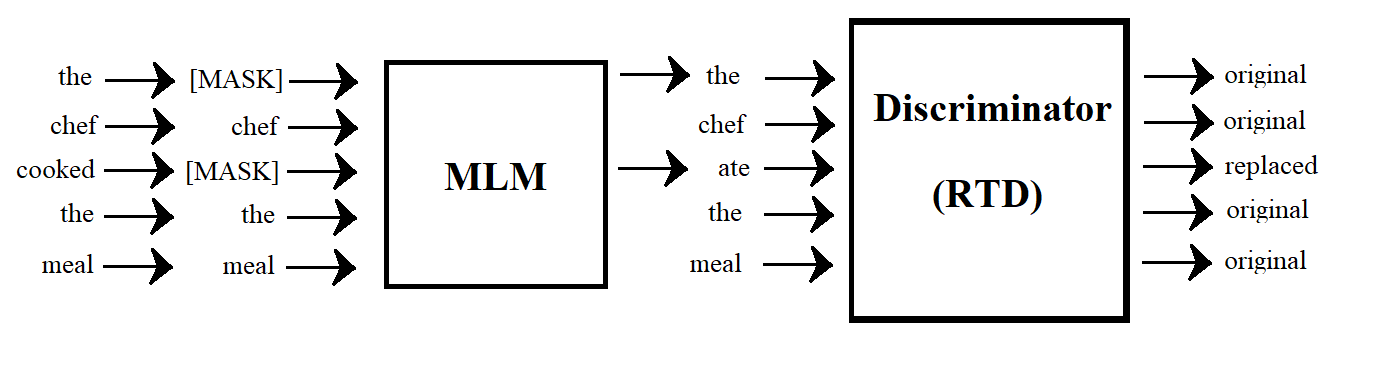
\includegraphics[width=9cm]{MLMRTD.png}
    \centering
    \caption{Graphical comparison between the MLM and the RTD tasks.}
\end{figure}

\subsubsection{GPT}
Recently, NLP algorithms employing pretrained GPT (Generative Pretrained Transformer) \cite{GPT} neural models have been gaining a lot of traction. Similarly to other state-of-the-art language models, GPT is a Transformer pretrained in a self-supervised manner for predicting the next token in a sequence. However, GPT combines unsupervised pretraining with supevised finetuning on a discriminative task, leading to improved internal representations.

Yet, when it comes to long-document NLP tasks, the latest openly available pretrained GPT model is GPT 2.0 \cite{GPT2}, which remains regularly outperformed by BERT-derived language models such as BART \cite{bart} and RoBERTa \cite{roberta} \cite{tanyangxing}. However, the size and amount of investment GPT models have attracted because of their text generative abilities and the publicity that came with it makes future GPT versions a serious competitor for BERT. %GPT 3.0 achieves similar results to most BERT-based language models \cite{tanyangxing}, but is not yet available to the public.

\section{Document Classification}
\label{sec::Classification}
Document Classification is the automatic assignment of one or more class labels to a piece of text, based purely on its contents and assuming a known finite set of discrete labels. In long-document NLP, the text in question is typically an entire document. As an example, a book of fiction could automatically be assigned a genre label by a text classifier deployed in a library, supporting labels such as ``Romance" or ``Science Fiction".

Overall, recent methods for neural long text/Document Classification mostly rely on pretrained Transformer language models (e.g., BERT) with a classification head appended at the end. The language model may be finetuned for the desired classification task, while training the head. This approach is suitable for most Document Classification tasks \cite{qian} \cite{ion} \cite{ion2} \cite{mcbert} \cite{ammar} \cite{so}. However Transformers may be suboptimal for specialized tasks or domains \cite{junhua}, allowing CNN and RNN architectures to occasionally outperform them on long documents. Relevant issues and solutions are discussed below.

\subsection{Challenges}
\label{ssec::ClassificationChallenges}
Long text classification algorithms inevitably face challenges that are common to all NLP tasks, as well as issues specific to the case of long texts. Below, follows a non-exhaustive list of the most significant relevant challenges:

\begin{itemize}
\item \textbf{Input size}. The size of the input document is the most significant challenge in long-document NLP. For example, the computational overhead of CNNs tends to grow proportionally to their inputs; thus, they are unable to process documents with thousands of sentences, without specialized hardware. On the other hand, RNNs/LSTMs struggle to conserve information and identify long-term dependencies over huge spans of text \cite{worsham_book}. Transformer DNNs, such as BERT and most of its variants, are typically constrained by a rather low maximum token sequence length; usually 512 or 1024 tokens. This limits their training to relatively short texts, forcing brutal token selection during inference. As a result, their performance on long texts is severely limited compared to shorter ones \cite{dai}. Additionally, traditional Transformer architecture \cite{ilia} rely on a global self-attention mechanism, comparing each token to all other input tokens, leading to a quadratic ($O(n^2)$) increase in both computational and, much more importantly, memory requirements with respect to input size. 

\item \textbf{The curse of dimensionality}. As the supported vocabulary increases in size, the possible inference-stage combinations of its words grow exponentially large, unlike the fixed training dataset size.

\item \textbf{Polysemy}. A word may express multiple different meanings in different contexts. For example the word ``bank" may mean a financial institution or a building. DNN models must learn to appropriately differentiate the exact meaning of a word depending both on the local context (sentence, paragraph) and the global context (document).

\item \textbf{Homonymy}. Homonyms are words that either share spelling (homographs), pronunciation (homophones) or both, but are not semantically related. For instance, the term ``bank" may refer to a financial institution or to the shore of a river. This example should clarify that the difference between homonymy and polysemy is that homonyms are not even related to each other in meaning.

\item \textbf{Figurative language}. Sarcasm, irony and metaphors pose serious challenges to NLP, since the real meaning of a phrase is different from the immediately obvious one \cite{Karamouzas2022}. Figurative language is common to both short and long texts, but in the latter case it can take the form of sustained allegories (particularly in literary books).

\item \textbf{Unstructured text}. Long texts may be very unstructured for the most part, while communicating information in rather indirect and abstract ways. For example consider a novel, partitioned in a few dozens of chapters, and contrast it with short texts, such as product reviews or tweets. In the first scenario, crucial information and layers of meaning may be distributed across a large number of very long chapters \cite{worsham}. Furthermore, long documents tend to follow constantly evolving textual and contextual conventions, leading to a higher chance of shifts between learnt and actual probability distributions. This is especially problematic for literary works, which are fluid and susceptible to changing cultural biases \cite{brazil}.

\item \textbf{Multiple labels}. In many cases, the longer an input document is, the more possible it becomes that it belongs to multiple classes concurrently. This fact requires algorithms which specifically take it into account for meaningful classification, since each document may have a varying numbers of ground-truth labels.

\item \textbf{Foreign language datasets}. Finally, another issue is the limited availability of training content for languages other than the most popular ones (e.g., English, French, Spanish, etc.). Given that both the word embedding networks and the main, task-specific NLP DNNs are typically trained on one language at a time, the lack of extensive datasets in rarer languages leads to less optimal embeddings and, as a result, reduced performance in downstream tasks. The situation is in fact even worse, due to limited training sets for the downstream tasks themselves. Thus, in the case of Document Classification for rare languages, less data-intensive machine learning algorithms may be preferred, such as decision tree classifiers \cite{brazil}, or alternatively the existing datasets can be artificially augmented \cite{geroge}.
\end{itemize}


\subsection{Solutions}
\label{ssec::ClassificationSolutions}

Traditional machine learning algorithms, such as Naive Bayes \cite{russel}, SVMs (Support Vector Machines) \cite{cortes} and ID3 decision trees \cite{quinlan} have been repeatedly applied for long Document Classification. In fact, they are still employed \cite{brazil} \cite{xu} and can be competitive even in large literary texts \cite{sicong}. However, the field has generally moved decidedly towards DNNs and this Subsection presents the relevant state-of-the-art. The innovations of the various existing approaches mostly fall under the following categories, which are more or less tied to the challenges mentioned in Subsection \ref{ssec::ClassificationChallenges}:


\subsubsection{Multi-label Classification}

Multiple labels are essential for many real-world applications \cite{hsu} \cite{patentnet}, thus many methods attempt to identify a document as belonging to multiple classes concurrently. This may be trivial to achieve in itself, using well-known DNN models that have been properly adapted. Class imbalance issues, which may lead to extremely biased patterns learned from the training data, and the varying number of labels per document can be handled by applying weighted loss functions. However, multi-label classification poses unique challenges with regard to how accuracy is measured.

One representative state-of-the-art approach attempting to tackle this scenario is \citet{sicong}, where multiple different classifiers (including a pretrained BERT) are comparatively evaluated in multi-label multi-class Document Classification, using the book genre recognition task as a benchmark.

The steps taken in \citet{sicong} to build a successful genre recognizer are telling of more general difficulties with long-document classification. Regarding the issue of multiple labels a modified accuracy metric was proposed and exploited to measure classification accuracy: the true positive and true negative classifier predictions were first computed separately per class label, with the proposed metric being the weighted average of correctness over all the label classes. Per-class weights were proportional to the class label frequency and normalized to sum to 1. Similarly, the employed loss function (Binary Cross Entropy) was modified to include weights for each label, so that each class is scaled inversely to the prominence of the class in the training set. 


\subsubsection{Feature Pruning}

This is the traditional way to handle long textual inputs. It involves systematically discarding as much text as possible at the preprocessing stage, while minimizing information loss. In order to cope with the potentially huge input size in long document analysis, almost all relevant NLP methods are prefaced by a preprocessing stage, where less useful input elements are removed. Appropriately reducing the input size improves both computational efficiency and accuracy. To this end, the book genre recognizer of \citet{sicong} uses an aggressive sampling method which first discards:

\begin{itemize}
    \item "stopwords", i.e., known, extremely frequent words such as "a", "and", "he", etc.,
    \item words that appear less than 20 times,
    \item words that appear in more than 75\% of all books,
    \item words that appear in more than 75\% of all classes,
    \item paragraphs where the frequency of the remaining words is less than a certain threshold,
    \item the contents of each remaining paragraph after the 512th token, because of technical limitations imposed by BERT.
\end{itemize}

Thus, each remaining paragraph is represented by a subset of its words that fall within a restricted, book-level set of "keywords". Finally, the sampled paragraphs are only those with the highest concentration of keywords. 

The goal of this ruthless sampling is to keep the input's length manageable for documents containing many thousands of pages. Methods similar or identical to this one are present in most NLP models specialized for long texts; thus, they are utilized extensively in most research cited in this paper.

On the other hand, the book genre recognizer of \citet{worsham} employs only minimal preprocessing, just enough to allow the DNN to run relatively efficiently. It relies on an index, consisting of the 5000 most common words from the supported vocabulary. No other preprocessing/sampling takes place, under the intuition that exposing the DNN to even statistically unimportant words facilitates an understanding of patterns and grammatical modifiers, such as tense and plurality. Words were represented by typical neural embeddings. Different strategies were evaluated for feeding the document to the classification DNN:
\begin{itemize}
    \item Feed only the first 5000 words of the document.
    \item Feed only the last 5000 words of the document.
    \item Feed only 5000 random words of the document.
    \item Feed the entire document, split into chapters.
    \item Utilize a traditional bag-of-words approach.
\end{itemize}

These strategies were then employed on a series of different architectures. Ultimately, the random word selection proved to consistently outperform other selection strategies for a multitude of classifiers, with the best performer being a CNN-Kim \cite{kim} architecture.

\subsubsection{Sparse Transformers}

Given the quadratic computational complexity of Transformer DNNs and their prominence in recent years, attempts have been made to reduce their cost. Such approaches try to achieve linear complexity with respect to the input size, by keeping track of a small, fixed-length window of neighbouring tokens around each input token, instead of considering all $n$ tokens for the attention heads. However, the unavoidable trade-off is a reduced ability of the DNN to capture long-term dependencies, which is as important for long texts as the complexity with respect to the input size.

\paragraph{The Sparse Transformer} The Sparse Transformer was introduced in \cite{sparse_attention}, so as to lower asymptotic complexity from $O(n^2)$ to $O(n\sqrt{n})$ by applying sparse factorizations to the base self-attention matrix of the Transformer. The goal was to effectively transform the costly self-attention operation to several small, optimized attention operations which sufficiently approximate the original mechanism. Additional optimizations, such as re-computation of attention weights during back-propagation to save memory, efficient sparse attention kernels and improved weight initialisation contribute to a less demanding architecture, which is thus able to handle longer sequential inputs.


 It is worth noting that the Sparse Transformer is a general model, capable of achieving competitive results in a number of deep-learning fields concerning very long input sequences, such as Image Density Modeling, Text Compression, Image Compression and Audio Sampling.

\begin{figure}
    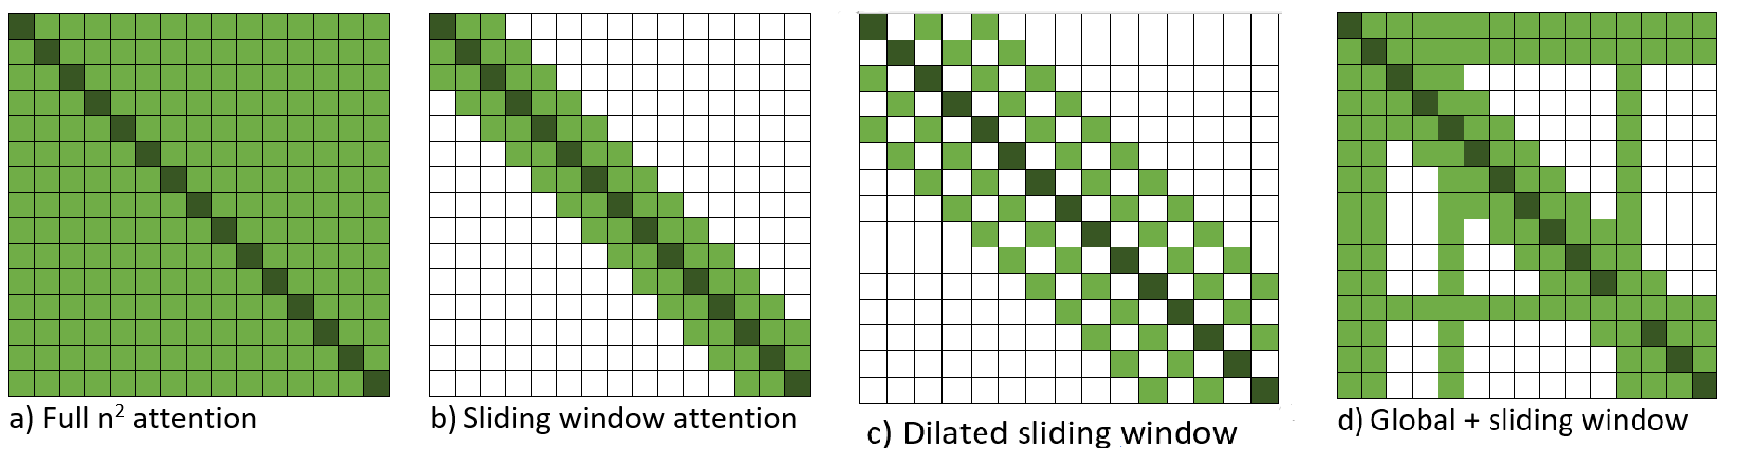
\includegraphics[width=12cm]{longformer.PNG}
    \centering
    \caption{Comparing the full self-attention pattern and the configuration of attention patterns in a standard Longformer.}
     \label{fig::longformer}
\end{figure}

\paragraph{Longformer} Surpassing the Sparse Transformer's computational gains, the Longformer \cite{longformer} achieves a linear asymptotic cost. Unlike the Sparse Transformer however, the Longformer is specialized for long-document NLP tasks. Notably, its self-attention mechanism can be used as a drop-in replacement for other Transformer models and operates by employing a \textit{dilated sliding attention window}, which is a modification of the classical sliding window approach. 

In typical sliding window implementations \cite{saeed, odysseas}, each token's window is comprised of $w$ tokens surrounding it: $\frac{w}{2}$ tokens to its left and right, respectively. The underlying intuition is that the semantic context of a token can be mostly derived from its neighbouring tokens, while the computational complexity of this operation is $O(n \times w)$. In NLP tasks the token is typically a word, but in the context of Transformers it is the position of that word in the self-attention matrix. The Longformer uses $l$ layers of self-attention in order to access tokens faraway from the original token.

The \textit{dilated sliding window} approach modifies the sliding window in order to allow efficient data analysis in large attention matrices. A sliding window of fixed size is moved over the data, with a predetermined dilation factor added at each step. The dilation factor determines the spacing between adjacent window positions and allows data analysis at multiple scales simultaneously. A larger range of tokens within the self-attention matrix can be covered, while avoiding redundant calculations and reducing computation time. Thus the receptive field of the window is of length $l \times d \times w$, while memory and processing costs remain steady.

Since windowed and dilated attentions may not be enough to extract a suitable sequence representation, certain additional, pre-selected locations of the full self-attention matrix are also allowed to be considered as global context. The number of these global tokens is kept constant and relatively small, so as to limit the self-attention mechanism's complexity to $O(n)$. A comparison between full, sliding, dilated sliding and global-dilated sliding window self-attention patterns is depicted in Figure \ref{fig::longformer}.

% \begin{figure}
%     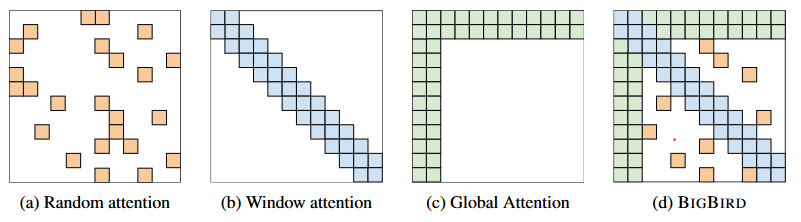
\includegraphics[width=12cm]{big_bird.PNG}
%     \centering
%     \caption{Figure 1: Building blocks of the attention mechanism used in BIGBIRD. White color indicates absence of attention. (a) random attention with r = 2, (b) sliding window attention with w = 3 (c) global attention with g = 2. (d) the combined BIGBIRD model. Image credits: \citet{big_bird}}
%      \label{fig::big_bird}
% \end{figure}

\paragraph{BigBird} Big Bird \cite{big_bird} can be seen as a variation of the Longformer, attempting to support much longer input sequences by reducing the complexity of self-attention from quadratic to linear. 

Similarly to the Longformer, the researchers also use a sliding window, as according to them, most contexts used in NLP tasks display great "locality of reference", meaning that the semantic context of a token can be mostly derived by its neighbouring tokens. Unlike Longformer however, instead of using a dilated sliding window in order to reach tokens far away from the original, the researchers use random token selection for each token's context. This complements the global attention and the regular sliding window attention schemes, adopted and adapted from the Longformer. It has been demonstrated mathematically that this modified sparse attention mechanism satisfies many theoretical properties of the original full-attention mechanism, such as universal approximation and Turing-completeness but seems to require more layers to retain accuracy comparable to full-attention architectures.

Additionally, Big Bird utilizes global tokens in two ways:
\begin{itemize}
    \item Some existing tokens are designated "global" in the internal transformer construction and are used in the entire sequence
    \item Other tokens are included as "global" with the same mechanism as Longformer in the external transformer construction. 
\end{itemize}

As such, the self attention mechanism has access to random tokens, tokens included in a sliding window, and to $g$ global tokens, some existing in the sequence, and some extra added as described above. %The token selection is showcased in Figure \ref{fig::big_bird}.

\subsubsection{Hierarchical Transformers}

Hierarchical models attempt to handle the large input size of long texts by appropriately building upon original Transformers, instead of modifying them. This is usually achieved in one of two ways:

\begin{itemize}
    \item By transforming the Transformer's input via a suitable DNN (e.g., a CNN or RNN/LSTM). The latter one generates a single document representation (document embedding) able to fit into a standard Transformer (e.g., BERT), thus bypassing the input size limitations.

    \item By segmenting the input document. The input segments are independently truncated to the Transformer's input size and the latter one (e.g., BERT) generates embeddings for each of these segments. A separate DNN then combines the segment embeddings and predicts the document label.
\end{itemize}

\paragraph{Hierarchical Attention Network} \citet{ion_han} were the first to build a Hierarchical Transformer architecture using a Hierarchical Attention Network (HAN) \cite{zichao} atop of a standard BERT. During inference, the input document is split into paragraphs that are truncated to fit into BERT. The latter one generates independent paragraph embeddings, which are combined by the succeeding HAN into a single output. The end result is an increased ability to handle long texts, by exploiting the natural partitioning of documents into paragraphs.

A similar approach was later used in \citet{glue_gunner}, where the base models were BERT, RoBERTa, DeBERT \cite{yanguang}, Legal-BERT \cite{ion6} and CaseLaw-Bert \cite{zheng}. In long text analysis tasks, the hierarchical versions proved competitive  with sparse-attention Transformers such as Longformer and Big-Bird. 

The method in \citet{khandve}, relying on BERT or on Universal Sentence Encoders (USEs) \cite{use} (models learning sentence representations for transfer learning), follows up on this methodology, but replaces the final HAN with a CNN or an LSTM architecture. The BERT+LSTM combination proved to be the best among the evaluated hierarchical approaches, but generally Hierarchical Transformers were outperformed by sparse-attention Transformers.

% \subsubsection{Hierarchical Transformers: Document Representations}

% \begin{figure}
%     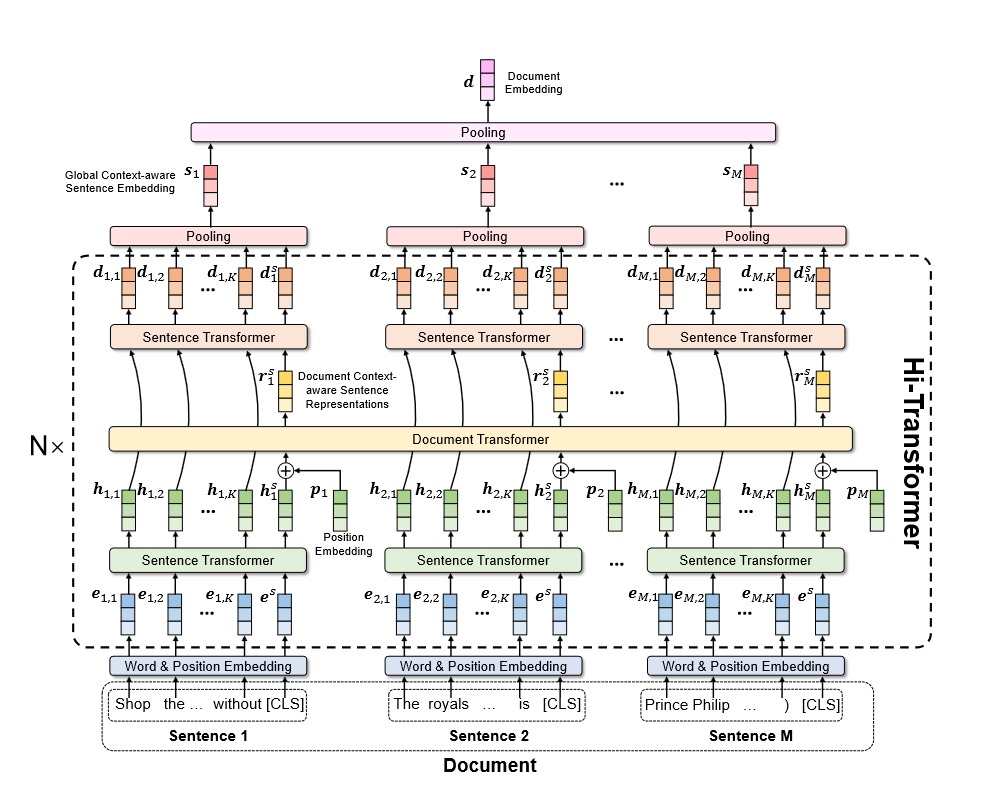
\includegraphics[width=12cm]{images/hi-transformer.PNG}
%     \centering
%     \caption{The architecture of Hi-Transformer. Image credits: \citet{qi}}
%      \label{hi-trans_fig}
% \end{figure}

\paragraph{Hi-Transformer} The main alternative to \citet{glue_gunner} and its variants is to essentially reverse the process, that is, to employ a hierarchical DNN for obtaining a fixed-length document-level representation/embedding from the entire input, which is then fed to regular Transformer. \textit{Hi-Transformer} \cite{qi} achieves this via a "Sentence Encoder", (in this model, a vanilla Transformer) which transforms the words of the input document into sentence embeddings. Once every sentence has been passed through the Sentence Encoder, these sentence embeddings are subsequently ordered using the model's positional embeddings and fed as input to a "Document Encoder" (again, a vanilla Transformer in this model). The latter's output is a context-aware document embedding, which is fed as input to the next Sentence Encoder so that it becomes aware of the global, document-level context. As a result, the generated sentence embeddings are aware of the global context. This process is repeated by stacking multiple such layers, until the final output is passed to a final pooling layer extracts the final document embedding. The researchers note that two layers seem to be sufficient, and further stacking does not yield significant improvements. % An overview of this approach is depicted in Figure \ref{hi-trans_fig}.

The Hi-Transformer has been shown to outperform sparse-attention Transformers in long text analysis tasks, which can be attributed to the readily accessible global/document-level context. Since BERT has to analyze a fixed-size document representation and the sentence encoder's complexity is linear to the number of sentences, computational demands are not higher than those of sparse-attention alternatives. Finally, the Hi-Transformer's accuracy in the desired downstream task (e.g., classification) tends in fact to increase with longer documents, since more relevant context can be extracted.


\paragraph{Hierarchical Sparse Transformer} Hierarchical Transformers have been combined with the sparse attention mechanism, in order to ameliorate the latter's inability to capture all the necessary global/document-level context, in the case of long texts, as well as its lack of robustness against small modifications to the input. The \textit{ERNIE-SPARSE} architecture \cite{liu} merges the two schools of thought by using hierarchical attention. which is then fed to a Sparse Transformer in order to increase the information extracted from the global context.

ERNIE-SPARSE consists of two distinctive parts; a Hierarchical Sparse Transformer (HST) and the Self-Attention Regularization (SAR) method.

The \textbf{Hierarchical Sparse Transformer} is a Transformer utilizing a modified Attention Mechanism which attends to a representative sample of the tokens in a fixed-length window, as well as global attention tokens, otherwise behaving as a standard Sparse Transformer. 

The \textbf{Self-Attention Regularization} is intended to make the sparse attention largely invariant to small changes in input. For it to be defined two distributions of the model need to be computed, $P_{1}(y|x)$ being the default sparse attention topology and $P_{2}(y|x)$ being the shifted attention topology. It thus defines a new loss function which attempts to minimize the Kullback-Leibler divergence between the original and a slightly shifted sparse attention output distributions. This loss function is then added to the standard negative log-likelihood loss function.

ERNIE-SPARSE has been shown to outperform RoBERTa, Longformer and Big-Bird on Document Classification tasks performed on the arXiv, IMDB and the Hyperpartisan datasets. 

It ιs worth noting that by our definition, ERNIE-Sparse can technically be considered a Sparse Attention model since it modifies the Transformer's internal architecture, despite this modification being inspired by Hierarchical networks.


\subsubsection{Recurrent Transformers}

Another recent proposal attempts to allow the Transformer's size to be arbitrarily increased during inference, regardless of training size, while maintaining linear cost complexity and local and global context retention.

%\begin{figure}
    %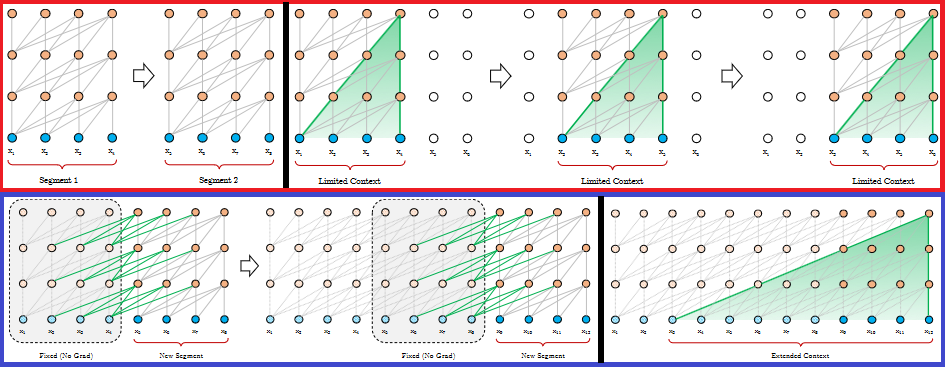
\includegraphics[width=14cm]{images/recurrent_comp.png}
    %\centering
    %\caption{Comparison between the base Transformer and Transformer-XL. Red: The base model. Blue: Transformer-XL. The black lines separate the training phase (left) and the evaluation phase (right). Tokens used for local context are shown in green. Image credits: \citet{dai-etal-2019-transformer}}
     %\label{fig::recurrent}
%\end{figure}

\paragraph{Transformer-XL} \citet{dai-etal-2019-transformer} originally propose a solution which aims to bypass the issue of context fragmentation and informational bottlenecks altogether. This is achieved by introducing "recurrence" within the self-attention network. They thus introduce their own Transformer architecture, called "Transformer-XL". Transformer-XL features two main modifications to the base Transformer model:
 
\textbf{Recurrence} is the method with which the model keeps a hidden memory for each segment of the input, which is then used in subsequent segments to transmit the previously established context. This architecture is inspired by the normal operations of RNN and LSTM networks, hence the term "recurrent". Unlike the recurrent mechanisms used in recursive DNNs, the recurrence mechanism in Transformer-XL shifts the dependency one layer downwards. For example, layer $l=n$ has access to 2 hidden states from layer $l=n-1$, 4 hidden states from layer $l=n-2$ and $2^n$ from layer $l=1$, which are the original word embeddings.

This mechanism guarantees $O(n \times l)$ cost, where $l$ are the number of layers, and a significantly faster evaluation of up to 1,800 times compared to the base Transformer model. It also allows a different model size to be used for training and evaluation, meaning that a model may be trained with a certain size, and evaluate documents with multiple times that size. %A comparison between this architecture and the base model can be found in Figure \ref{fig::recurrent}.

\textbf{Relative Positional Embeddings}. The original Transformer model uses Absolute Positional Embeddings, allowing it to order all words in the input sequence. As this is mathematically incompatible with the modifications shown above (because of the reused states), the researchers defined and used Relative Positional Embeddings instead. These embeddings are used to codify the distances between the segments, rather than how to order them. This distance is then injected into the attention score. 

Ultimately, Transformer-XL achieves competitive results on long-document datasets with traditional model, and models utilizing the base Transformer architecture, at a much more efficient cost.


\paragraph{ERNIE-Doc} \citet{ernie-doc} build upon the work of \citet{dai-etal-2019-transformer} by proposing ERNIE-Doc, a recurrent Transformer which makes two passes over the input, similar to how humans first "skim" a document before paying attention to important sections.

The way they achieve this is by computing the cached hidden state as follows:
\begin{equation}
    \hat{H} = [\hat{H}^{1}_{1:T};...;\hat{H}^{N}_{1:T}] \text{(skim phase)}
\end{equation}

\begin{equation}
    \tilde{h}_{r+1}^{n-1} = [SG(\tilde{H};h_{r+1}^{n-1})] \text{(retrospective phase)}
\end{equation}

where $\tilde{H} \in \mathbb{R}^{L\times T\times N \times d}$ are the cached hidden states from the skimming faces for $T$ segments each, $\hat{H}^{1}_{1:T} = [\hat{h}^{i}_1;...;{h}^{i}_T]$, $L$ is the length of the document and $N$ is the number of layers.

This skimming architecture is incompatible with the recurrence mechanism introduced in \citet{dai-etal-2019-transformer}. Additionally, because of its linear dependency with regard to the number of layers, the computational and memory costs of the Recurrence mechanism can be prohibitive for long documents. To solve this, the researchers introduce an \textbf{"Enhanced Recurrence Mechanism"}. This mechanism "flattens" the hidden state dependency from one-layer-downwards recurrence to same-layer recurrence similar to recursive DNNs.

The researchers also define a new learning objective called "Segment-Reordering Objective" for pre-training. This document-aware task entails splitting a long document in $m$ chunks, shuffling them, then letting the pre-trained model reorganize them. The model was pretrained on this task and the common Masked Language Modeling (MLM) task \cite{toutanova} using a combination of the Wikipedia, BooksCorpus \cite{kiros}, CC-News and Stories \cite{trinh} datasets, tokenized using ROBERTa \cite{roberta}.

ERNIE-Doc has been proven to produce competitive results, comparable to Big-Bird and the Longformer on Document Classification, Document-level Question-Answering and Keyphrase-Extraction tasks on various long-document datasets.


\subsection{Sparse or Hierarchical Transformers?}
These two approaches of solving the inherent limitations of the Transformers' original architecture have dominated current research on Long-Document NLP models. However both suffer from unique challenges:

Sparse Attention Transformers tend to suffer from what \citet{liu} call "informational bottlenecks", where the models are forced to rely on a small number of global tokens to encapsulate global document context. They also suffer from a lack of input invariance, making them susceptible to be "fooled" by minor changes in the input text.

Hierarchical Attention Transformers on the other hand struggle with loss of information because of the split of the input document. This is usually the result of context fragmentation, where these segments are either lacking sufficient local context \cite{dai}, or have no access to the document's global context \cite{qi}.

As these two techniques mature and evolve both in parallel, and in competition with each other, their respective challenges will most likely be solved. However, as of writing, there is no consensus on which performs better, nor any empirical rule on which tasks each architecture performs best in. 
 

\section{Document Summarization}
\label{sec::Summarization}

Automatic Text Summarization (ATS) is the task of generating a short summary from a given document. It is often called "Document Summarization", especially in the context of long documents (such as medical and legal records). Importantly, the generated text must be coherent, while accurately maintaining the meaning of the most important information in the source material. There are two main approaches to ATS; \textit{extractive} and \textit{abstractive} summarization.

\textbf{Extractive summarization} generates its summary using verbatim sentences found in the source text. This practically reduces summarization into finding a binary selection vector $\mathbf{s} = [s_1, s_2,..., s_n]^T, s_i \in \{0,1\} \forall i \in [1,n]$, where $s_i = 1$/$s_i = 0$ if the $i$-th original input text sentence is/is not to be included in the summary, respectively. As such, this approach offers easy summary generation from both an algorithmic and a computational perspective. Extractive summarization is therefore very common, especially for summarizing on-line articles. However, its applicability is inherently limited in the sense that not all document types can be summarized well by just a few of their sentences taken verbatim and re-arranged. For example, there is no way to describe the content of most books by using a selection of their own sentences. Additionally there are concerns that simple extractive approaches are reaching their peak, and thus research must gravitate towards: a) ensembles of multiple extractive models, or b) abstractive summarization methods \cite{mehta}.
	
\textbf{Abstractive summarization} is the alternative approach of generating new text. It is the method humans use when trying to manually summarize text, by reading the source, extracting its meaning and then writing a condensed document which contains as much of the original's meaning as possible. Modern abstractive algorithms mostly are DNNs following an Encoder-Decoder architecture \cite{cho}. Compared to extractive summarization, this approach generates a more meaningful and condensed summary, while being more adaptable to the input document's type. However, there is a much larger risk of misrepresenting facts, and of the output summary not being coherent at all. The most commonly used method for abstractive summarization involves employing a Seq2Seq model, as introduced by \citet{seq2seq}. This model follows an encoder-decoder architecture, utilizing either recurrent neural networks (RNNs) as proposed by \citet{LSTM} or, more recently, transformers as presented by \citet{ilia}. Within this model, the encoder captures the underlying representations of the given tokens (words or subwords) in the document, based on which the decoder generates a summary.

	
\subsection{Challenges}
\label{ssec::SummarizationChallenges}
Document Summarization comes with its own set of challenges. These are essentially specific to the case of long texts, since there is typically no reason to summarize a short text, but a subset of them are shared with the challenges faced by long-document classifiers.

\begin{itemize}
    \item \textbf{Input size}: The length of the input document gives rise to significant issues which go beyond simple computational and hardware requirements. Extractive DNNs particularly struggle with long documents \cite{xiao}; the greater the length of the input, the more topics it typically covers, thus the harder it is for a DNN to generate a summary covering effectively all of them.

    \item \textbf{Metrics}: The ROUGE evaluation metric \cite{rouge}, which is the most commonly used metric for summarization tasks, might not be sufficient for abstractive DNNs. It has been claimed that it performs considerably worse in abstractive DNNs since it lacks semantic understanding of the words it compares. Indeed, the ROUGE metric may not even be sufficient for extractive summarization \cite{akter}.

    \item \textbf{Sentence extraction}: Framing extractive summarization as a binary decision task assumes that the meaning of individual sentences is independent from that of others, leading to high redundancy. Even accounting for this fact, such DNNs are still vulnerable to greedily picking general sentences, instead of finding a combination of specific sentences which together summarize the document much more effectively \cite{matchsum}.

    \item \textbf{Repetition}: One of the most common issues of abstractive DNNs dealing with long texts is sentence repetition; this is potentially caused by the over-reliance of a Decoder to its input, which gives rise to an endless loop of phrase repetition \citet{abigail}. Internal issues concerning RNNs with attention mechanisms have been pointed out as the root cause of both this issue and of false information appearing in the output summary \citet{suleiman}.

    \item \textbf{Transformer issues}: Most relevant state-of-the-art deep neural architectures feature the Encoder-Decoder pattern, implemented via Transformers. The challenges plaguing Transformer architectures such as BERT have already been largely analyzed in Section \ref{ssec::ClassificationChallenges}. Many of these remain equally critical issues in long-Document Summarization as well.
\end{itemize}
	
	
\subsection{Solutions}
This Section reviews the evolution of extractive and abstractive models, as well as how each family attempted to handle the challenges it faces.

Fist, the ROUGE score is discussed, along with the reasons for its prominence, its weaknesses and some of its alternatives in \textbf{Evaluation Metrics}. Subsequently, extractive and abstractive summarization DNNs are examined in separate sections.
    

\subsubsection{Evaluation Metrics}
ROUGE is a very commonly used metric for evaluating ATS tasks and therefore features as many as 192 variations. The base ROUGE metric \cite{rouge} measures the number of overlapping n-grams/sequences between the generated and ground-truth summary. This is sufficient for many extractive summarization tasks, but faces severe challenges when used for abstractive summarization. For instance, ROUGE is unable to distinguish between different grammatical versions of the same word \cite{suleiman} and synonyms \cite{akter}. ROUGE is also agnostic towards sentence ordering \cite{graham}. Most importantly, perhaps, the underlying assumption made by ROUGE, where the quality of a summary is correlated to its coverage compared to the human-generated summary, may not be statistically significant \cite{pitler}.

The reasons why ROUGE is still used as the default metric despite such severe drawbacks are multiple, including the unavailability of similar metrics and the lack of easy-to-use toolkits \cite{fabbri} (libraries, datasets, models and pipelines intended for use in comparing and evaluating metrics). Besides, alternative metrics may suffer from similar weaknesses, since they are typically configured on the same, biased datasets \cite{kryscinski}. For a detailed discussion of text summarization metrics, the reader is suggested reference \citet{fabbri}. For the purposes of this article, a number of common and/or recent alternatives to ROUGE are briefly mentioned below:

\begin{itemize}
    \item METEOR \cite{meteor} (recommended by\citet{suleiman}), functions similar to ROUGE, while being largely invariant to grammatical variants and synonyms.
    \item Sem-nCG \citet{akter} is a recent, semantically-aware metric focused on \textit{extractive} summarization.
    \item BERTScore \cite{bert_score} uses the similarity of the contextual embeddings between the generated and ground-truth summaries.
    \item $S^{3}$ \cite{s3} combines other evaluation metrics through a model, in order to produce an aggregated evaluation of the summary.
    \item BLANC \cite{blanc} is an unsupervised evaluation metric which does not depend on human-generated summaries, by exploiting NLP tasks.
\end{itemize}
This is by no means an exhaustive list of evaluation metrics. It is meant to demonstrate that the question of a capable successor to ROUGE is still an open one.

\subsubsection{Extractive summarization approaches}
\label{sssec:extractive}
This section presents the gradual evolution of extractive summarization DNNs towards the current state-of-the-art.\\

\paragraph{Building Summaries Using Hierarchies} We discuss the first attempts using DNNs to achieve extractive and summarization. These models, while certainly obsolete today, describe the core concepts of ATS which were then largely re-used and improved.

%\begin{figure}
        %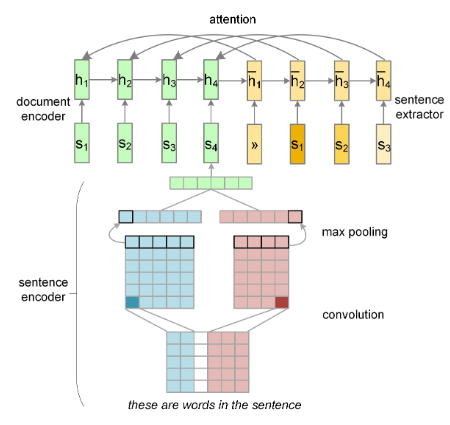
\includegraphics[width=10cm]{summarization-rnn.PNG}
        %\centering
        %\caption{ A recurrent convolutional document reader with a neural sentence extractor Image credits: \citet{lapata}}
        %\label{lapata_fig1}
    %\end{figure}

   % \begin{figure}
        %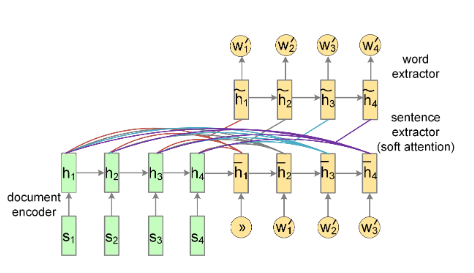
\includegraphics[width=10cm]{summarization-rnn2.PNG}
        %\centering
        %\caption{ Neural attention mechanism for word extraction. Image credits: \citet{lapata}}
        %\label{lapata_fig2}
   % \end{figure}
	
The method in \citet{lapata} developed a neural Encoder-Decoder architecture, augmented with an attention mechanism, to tackle extractive summarization. 

The Encoder relies on two DDNs; a CNN model called "Convolutional Sentence Encoder" which obtains sentence embeddings and a LSTM model called "Recurrent Document Encoder" which takes these embeddings as input and produces a document embedding, effectively deriving the meaning of a document from its constituent words. 

The Convolutional Sentence Encoder's inputs are $d$-dimensional word embeddings. These embeddings were initialized using the word2vec embeddings \cite{mikolov}. Its operations are computed as does a typical CNN using multiple feature maps and kernels of different widths. This produces many alternative sentence vectors which are then summed up and given as output.

The Recurrent Document Encoder's parameters were randomly initialized using the Uniform Distribution. It otherwise functions as a typical LSTM model, with its hidden states used by the Decoder as described later on.

The Decoder is one of two models following different strategies; a \textit{Sentence Extractor}, which approaches the extraction task as a sentence selection problem, and a \textit{Word Extractor} which approaches it as a word generation task. These models are mutually exclusive and trained and evaluated on different datasets both based on the CNN/Daily Mail dataset (See Section \ref{sec::Datasets} for details on the dataset).

The Sentence Extractor is a LSTM model sequentially selecting sentences based on two criteria; whether they are relevant, and whether they are mutually redundant with other sentences. The selection decision is computed as follows:

\begin{equation}
    \mathbf{\hat{h}_t} = LSTM(p_{t-1} \mathbf{s_{t-1}}, \mathbf{\hat{h}_{t-1}}
\end{equation}

\begin{equation}
    p(y_L(t) = 1 | D) = \sigma(MLP(\mathbf{\hat{h}_t}; \mathbf{h_t})) 
\end{equation}
where $\mathbf{\hat{h}}$ are the encoder hidden states, $\mathbf{h}$ are the extractor hidden states, $t$ is the current time-step, $p_{t-1}$ represents the assigned probability that the previous sentence should belong to the summary and $;$ is the concatenation operation.

The Word Extractor on the other hand is practically an Abstractive Summarizer with its vocabulary constrained to that of the input document, limiting its efficiency. Since its architecture was never subsequently used, we will not provide details on its operation in this paper.

The datasets used for either of the Decoders are adapted from the CNN/Daily Mail dataset. The extractive dataset for the Sentence Encoder is generated by selecting the sentences which feature the most semantic similarity with the ground-truth summary. The dataset for the Word Extractor on the other hand, was generated by selecting the words with the highest lexical overlap between the highlights (ground-truth summary sentences) of the article with Out Of Vocabulary (OOV) words being replaced by the most semantically equivalent word in the article.

Following-up on the hierarchical Encoder-Decoder framework introduced by \citet{lapata}, \citet{nallapati} propose SummaRuNNer, an extractive, RNN-based sequence classifier, equipping it with a training mechanism that allows it to train on abstractive ground-truth summaries.

The model runs on multiple layers of bi-directional GRU-RNNs. Similarly to \citet{lapata}, the model uses a 2-layer Encoder framework; the first layer to produce sentence embeddings from words, and the second layer to produce document embeddings from the sentence embeddings. The Decoder is made of a simple logistic layer. 

The sentence representation produced by the first layer follows the typical GRU-RNN training and inference operations. The document representation of the model is the average pooling of the second level's hidden states described as follows:

\begin{equation}
    d = tanh(\mathbf{W_{d}} \frac{1}{N} \sum^{N^{d}}_{j=1}[\mathbf{h^{f}_{j}};\mathbf{h^{b}_{j}}] + \mathbf{b})
\end{equation}
where $\mathbf{h^{f}_{j}}$ and $\mathbf{h^{b}_{j}}$ are the hidden states corresponding to the $j$th sentence of the forward and backward sentence-level RNNs respectively, $N^{d}$ is the number of sentences in the document and ‘;’ represents vector concatenation. 

The Decoder then classifies documents taking into account the salience, novelty as well as the absolute and relative positional embeddings of the content.

The model can be trained via extractive training, on datasets where the summary is a binary vector, where $1$ means a sentence needs to be included and $0$ that it should be skipped, and on abstractive summaries. This allows the model to train on many datasets which feature human-generated summaries without further pre-processing, which was the case in \citet{lapata}.

In the case of an extractive dataset the loss function is a standard CrossEntropyLoss function between the predicted and ground-truth binary summary vectors. Otherwise, a RNN decoder is placed on the Encoder \textit{only} during training time, emitting the most probable word at each time-step. 



%\begin{figure}
%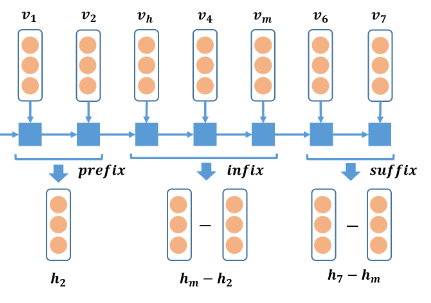
\includegraphics[width=10cm]{summarization-lstm.PNG}
%\centering
%\caption{ Illustration for learning segment embeddings based on an extra forward LSTM network, $\upsilon_{h}, \upsilon_{b}$ and $\upsilon_{1}$ to $\upsilon_{7}$ indicate the output vectors of Bidirectional LSTM for head word h, modifier word m and other words in sentence, $h-{h}, h_{m}$ and $h_{1}$ to $h_{7}$ indicate the hidden vectors of the forward LSTM corresponding to $\upsilon_{h}, \upsilon_{m}$ and $\upsilon_{1}$ to $\upsilon_{7}$ Image credits: \citet{wang}}
 %\label{wang_fig}
%\end{figure}

\citet{xiao} improve on the solutions provided by \citet{lapata} and \citet{nallapati} by incorporating local and global context information found in the document. This approach was inspired by the hierarchical structure that most human documents of significant length use, and it was thus hypothesized hierarchical information would be especially beneficial for long documents. 

This is achieved by using the LSTM-minus technique\cite{wang} in an attempt at producing context-aware embeddings. We will refer to this model as "LSTM-Ext" for the purposes of this paper. The technique is applied on the document level in order to discover the sections and topics of a given document. Similar to \citet{lapata} and \citet{nallapati}, the model uses an Encoder-Decoder framework, where the Encoder is composed of a sentence and a document encoder, as well as a topic encoder which provides access to local context. The model thus operates as follows:

\begin{enumerate}
    \item The sentence encoder maps word embedding to a fixed length vector. 
    \item  The document encoder uses a bi-directional RNN to encode the sentences.
    \item The topic encoder then embeds information about a sentence's topic.
    \item  The decoder produces the summary, by choosing whether to concatenate the sentence vectors produced by the document encoder, then using an attention mechanism to assign weights to them and finally passing them to a sigmoid layer which chooses whether to include them in the summary.
\end{enumerate}

The sentence encoder is computed with standard GRU operations. The document encoder is computed by concatenating the final state of the forward and the backward GRU. The topic encoder is composed of bi-directional GRUs following the LSTM-Minus technique proposed by \citet{wang}.

The decoder then selects sentences by concatenating the document, optionally assigning weights using an attention mechanism, and then passing the merged representation in a final MLP followed by a sigmoid activation function. 

The LSTM-Ext model was trained on the arXiv and Pubmed datasets, using pre-trained GloVe \cite{glove} word embeddings (see Section \ref{sec::Datasets}). Their model's efficiency seems to increase with samples of ever increasing document length, making it a powerful architecture for long documents. 


\paragraph{Hierarchical Summaries using BERT}. We showcase the jump from traditional DNNs to todays Transformer models, from Vanilla to BERT and later to specialized variants. We observe how each iteration implements older ideas to improve its efficiency and how the various challenges of long documents are resolved.\label{sssec: HierBERT}

\citet{lapata_bert} use BERT models\cite{toutanova} (See Section \ref{sec::DNNs}) for both Extractive and Abstractive Summarization tasks, called BERTSUM-EXT AND BERTSUM-ABS respectively. Instead of using sentence representations, as previous research analyzed in Section \ref{sssec:extractive}, BERT inherently uses token representations. The researchers thus insert special tokens in-between sentences to signal to the model that those token segments are distinct sentences. They also use randomly initialized position embeddings in order to overcome BERT's maximum length of 512.

BERTSUM-EXT uses the Encoder-Decoder framework described in the previous section, where a sentence encoder produces sentence embeddings, which are then fed to a document encoder, which produces an embedding for the whole document. Specifically, the model feeds BERT's outputs to multiple inter-sentence Transformer layers whose task is to produce a document embedding, which is finally passed to a standard sigmoid layer for classification.

The model was trained on the CNN/Daily Mail, NYT \cite{nyt_dataset} and XSum \cite{nallapati2} datasets which feature primarily short-to-medium length documents. The model performed exceptionally but met the same challenges as all Transformer-based models on longer documents. An approach used by \citet{histruct}, much more reminiscent of the LSTM-Ext model, uses a separate model (HiStruct) which determines the hierarchical structure of the input text and injects it into an extractive summarization model (\textbf{HiStruct+}). The extractive summarization model can be implemented by multiple transformer-based architectures, such as BERT, RoBERTa and Longformer.

The HiStruct model encodes the hierarchical position of a sentence as 
\begin{equation}
\label{eq::hier_pos}
    SSV_{\mathbf{s}} = (\mathbf{a}_{s}, \mathbf{b}_{s})
\end{equation}
where $a_{s}$ represents the linear position of the section containing the sentence and $b_{s}$ is the linear position of the sentence with that section. The resulting matrix guarantees that all sentences within the same section are spatially proximal to one another, as are sentences that are close to one another in a section. 

The HiStruct+ model on the other hand, replaces the traditional Position Embeddings with Hierarchical Position Embeddings, which calculate the distance of any two tokens on the two-dimensional position matrix introduced in Equation \ref{eq::hier_pos}. 

The model seems to perform exceptionally well in long documents with a rigid hierarchy, such as the arXiv and Pubmed datasets, while still achieving SOTA results in short-to-medium length datasets such as the CNN/DailyMail dataset.


\paragraph{HyperGraph Transformers} HyperGraph Transformers are a novel approach to Extractive Summarization, combining ideas from models in \textit{Building Summaries Using Hierarchies} and implementing them using Graph Neural Networks (GNNs).

 %\begin{figure}
    %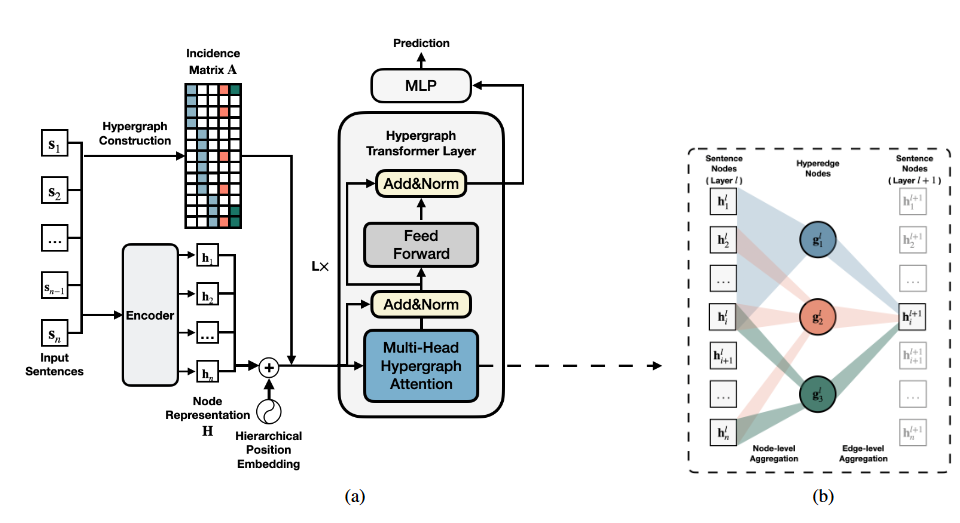
\includegraphics[width=12cm]{images/hegel2.PNG}
    %\centering
    %\caption{(a) The overall architecture of HEGEL. (b) Two-phase message passing in hypergraph transformer layer. Image credits: \citet{hegel}}
    %\label{fig::hegel}
%\end{figure}

\citet{hegel} attempt to deal with the Transformer's quadratic complexity and context retention problems by utilizing a Graph Neural Network (GNN) approach. They propose a new model, \textbf{HEGEL}(HypErGraph transformer for Extractive Long Document Summarization) which represents any document as a graph with hyper-edges including information about the section structure, current topic and keywords respectively. 

HEGEL models the document as a graph, i.e a graph $G = (V, E)$ where $V$ is a set of nodes and $E$ a set of hyperedges (an edge that can connect two or more nodes). We use the notations $u \in e$ and $u \notin e$ to represent whether a node is connected to a hyperedge in graph $G$ or not respectively.

There are three kinds of hyperedges in the document graph:
\begin{itemize}
    \item \textbf{Section Hyperedges} is a hyperedge which connects all sentences that belong to the same section. In the context of a scientific article, a section could be the problem, methodology and conclusions. We can thus build an incidence matrix $A^{sec}$ as:

    \begin{equation}
     \mathbf{A}^{sec}_{i,j} =
      \begin{cases}
          1, \text{ if } s_{i} \in e^{sec}_{j} \\
          0, \text{ if } s_{i} \notin e^{sec}_{j}
      \end{cases}
    \end{equation}
    where $s_{i} \in e^{kw}_{j}$ means the $i$-th sentence belongs in the $j$-th section.

    \item \textbf{Topic Hyperedges} is a hyperedge which connects all sentences which share the same topic. The topic clustering is implemented by using Latent Dirichlet Allocation \cite{dirichet}. We thus define incidence matrix
    $\mathbf{A}^{topic}$ as:
    
     \begin{equation}
     \mathbf{A}^{topic}_{i,j} =
      \begin{cases}
          1, \text{ if } s_{i} \in e^{topic}_{j} \\
          0, \text{ if } s_{i} \notin e^{topic}_{j}
      \end{cases}
    \end{equation}
    where $s_{i} \in e^{kw}_{j}$ means the $i$-th sentence belongs in $j$-th topic.

    \item \textbf{Keyword Hyperedges} is a hyperedge which connects all sentences which contain the same keywords. These keywords are extracted using Key-BERT \cite{keybert} from the training sample. We thus define incidence matrix $\mathbf{A}^{kw}$ as:

    \begin{equation}
     \mathbf{A}^{topic}_{i,j} =
      \begin{cases}
          1, \text{ if } s_{i} \in e^{kw}_{j} \\
          0, \text{ if } s_{i} \notin e^{kw}_{j}
      \end{cases}
    \end{equation}
    where $s_{i} \in e^{kw}_{j}$ means the $i$-th sentence contains the $j$-th keyword.
\end{itemize}

We can build the overall incident matrix $A \in \mathbb{R}^{n\times m}$ by concatenating the three incidence matrixes as:
\begin{equation}
    \mathbf{A} = \mathbf{A}_{sec};\mathbf{A}_{topic};\mathbf{A}_{kw}
\end{equation}

The researchers proceed to define a new Transformer architecture based on hyperedge input features called \textbf{Hypergraph Transformer}, upon which HEGEL is based. They begin by defining an alternative "Hypergraph Attention" mechanism using the Hierarchical Position Embeddings introduced in Section \ref{sssec: HierBERT} by \citet{histruct}. This is subsequently used to define the respective "MultiHead HyperGraph Attention" Mechanism, mimicking the one used in vanilla Transformers.  

The MultiHead HyperGraph Attention is combined with standard Feed-Forward Networks (FFN), standard residual connections and layer normalization mechanisms to create the Hypergraph Transformer. This new model additionally utilizes a distinct training algorithm utilizing a standard BCE loss function. 

%An abstracted view of the model can be found in Figure \ref{fig::hegel}.

HEGEL manages to outperform all extractive and abstractive baselines on both arXiv and CNN/Daily Mail datasets, demonstrating the potential of GNNs for long Document Summarization. It remains to see if similar models can retain this performance on less rigid and hierarchical document types however.


\subsubsection{Abstractive Summarization}

\paragraph{Pointer Generated Networks} We begin by discussing one of the first truly successful abstractive summarizers, which uses a hybrid approach combining extractive and abstractive techniques to create a model which can choose whether to copy, or generate the next word in the summary. 

%\begin{figure}
    %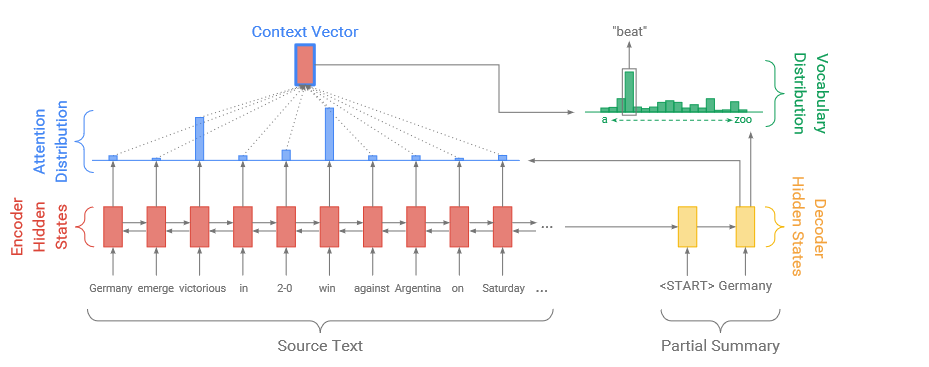
\includegraphics[width=12cm]{summarization-pointer1.png}
    %\centering
   % \caption{Baseline sequence-to-sequence model with attention. The model may attend to relevant words in the source text to generate novel words, e.g., to produce the novel word "beat" in the abstractive summary "Germany beat Argentina 2-0". Image credits: \citet{abigail}}
    %\label{abigail_fig1}
%\end{figure}

%\begin{figure}
    %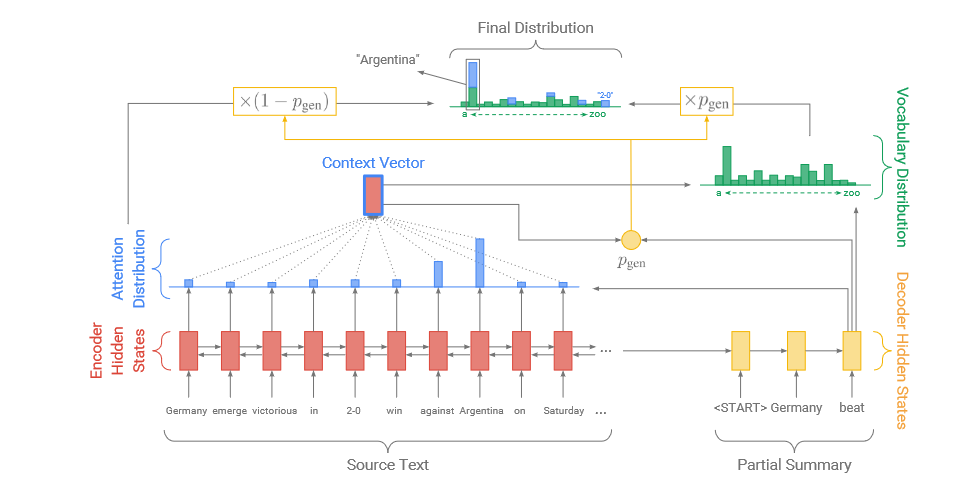
\includegraphics[width=12cm]{summarization-pointer2.png}
    %\centering
    %\caption{ Pointer-generator model. For each decoder time step a generation probability $p_{gen} \in [0, 1]$ is calculated, which weights the probability of generating words from the vocabulary, versus copying words from the source text.  Image credits: \citet{abigail}}
    %\label{abigail_fig2}
%\end{figure}

\citet{abigail}, propose a new solution to the word copying problem mentioned above by using "pointer-generator networks". Inspired by the ability of mammals, including humans, to refer to objects they do not know by pointing at them, pointer-generator networks may choose whether to generate a word, or copy it from the source text. This effectively makes the network a hybrid of extractive and abstractive models, and a practical application of the "Word Extractor" proposed by \citet{lapata}. 

An important strength of the network is that it can copy out-of-vocabulary words, which makes it possible to generate text with rare words, as well as keep a smaller vocabulary, thus reducing computational and memory costs. This effectively creates a hybrid model, leveraging the strengths of both summarization approaches. This is also the defining difference between this approach and the previously mentioned "Word Extractor" \cite{lapata}. 

The model uses a modified sequence-to-sequence Encoder-Decoder framework implemented similarly to that of \citet{nallapati}. Both the Encoder and the Decoder are one-layer, bi-directional LSTMs. The Decoder however, instead of selecting sentences by generating binary vectors, generates a new word originating either from the source document or an extended, global vocabulary. 

The attention distribution is defined as in \citet{bahdanau} and a coverage matrix is built and updated for each time-step, which penalizes the model for giving attention to  already extracted words. In order to decide on the course of action for the next word, the model obtains the probability distribution over the union of the global and the document's vocabulary (called the "extended vocabulary") and uses it to decide whether or not it should copy or generate the next word. The mechanism guarantees that if a word $w$ is OOV, the word will be copied from the source document, while if it does not exist in the document a new word will be generated.

The model does not use any pre-trained embeddings, learning word representations from scratch using the CNN/Daily Mail dataset. The model had remarkable success in handling OOV words, while also featuring a smaller vocabulary size and faster training times. It thus successfully handled most of the challenges outlined in Section \ref{ssec::SummarizationChallenges}. It was however not tested nor used on long Document Summarization, which is why more efficient and specialized models had to be developed.


\paragraph{BERT \& Sparse Attention Transformers}  In Section \ref{sssec:extractive} we featured \citet{lapata_bert} who adapted the Encoder-Decoder framework for Extractive Summarization tasks using BERT models. This same architecture and framework were used in the same paper to build an Abstractive Summarization model called \textbf{BERTSUM-ABS}.

The Encoder is a pre-trained BERTSUM model. They also propose using a pre-trained BERTSUM-Ext model (i.e the model used for extractive summarization) as the encoder, in which case they call the model \textbf{BERTSUM-EXT-ABS}. They thus hoped to realize efficiency gains from a transfer-learning approach, as well as task-specific gains between extractive and summarization tasks \cite{wei2, gehrmann}.

The Decoder is an \textit{untrained} 6-layer Vanilla Transformer. The researchers note that the untrained decoder may prove unstable during training and thus propose training the encoder and decoder on separate schedules. Specifically, they propose a slower learning rate for the pre-trained Encoder, in order for it to not be drastically destabilized by an unstable Decoder. The Encoder's learning rate would then gradually increase, as the Decoder became more schedule.

The datasets used were already described in the previous section. BERTSUM-ABS did indeed realize performance gains compared to other models, although it was proven that the BERTSUM-EXT-ABS variant only managed marginal performance gains.

In Section \ref{ssec::ClassificationSolutions} we discussed the reasons Vanilla Transformers can not be efficiently used for very long documents. The biggest challenge proved to be the self-attention mechanism and its $O(n^{2})$ cost in memory and computation.

We also discussed a modification to these models which attempted to bypass this restriction, those being Sparse Transformers. Most of these models can be dropped-in traditional extractive and abstractive summarization tasks by substituting the Encoder part of the summarizer. Below are two successful examples of Sparse Transformers being used for Document Summarization.

The \textbf{Longformer-Encoder-Decoder(LED)} model is a Longformer variant which features both encoder and decoder stacks, instead of just the encoder, and where instead of a full-attention mechanism, the encoder uses the local+global attention mechanism described in Section \ref{ssec::ClassificationSolutions}. The decoder utilizes full-attention to the entire encoder and to already-decoded positions of the input. 

As with its standard configuration, the LED scales linearly with the input size, and has been proven to achieve as-of-then state-of-the-art results in the arXiv dataset.

The \textbf{Big Bird} architecture \cite{big_bird} is a state-of-the-art Sparse Attention Transformer model. As in the case of Longformer, Big Bird can be used for \textit{abstractive} Document Summarization using an encoder-decoder architecture.

Specifically, Big Bird's sparse attention mechanism is used in the encoder part of the model, as that part is responsible for handling the large input and is thus memory and computationally expensive. The decoder part uses full self attention as the output length of the summary is significantly reduced.

The researchers' experiments show significant performance gains on large-document datasets, and competitive performance on smaller document datasets.


\paragraph{Local Attention and Content Selection} We showcase a state-of-the-art model which combines model and oracle-based feature selection and BART Transformers to efficiently produce abstractive summaries on long documents.

%\begin{figure}
    %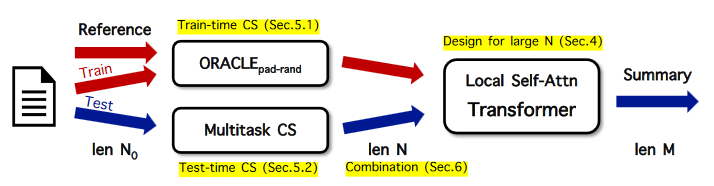
\includegraphics[width=10cm]{images/local_context.png}
    %\centering
    %\caption{ Overview of the combined architecture where we highlight different aspects of this work. $N_0$ is the original document length, N is the input length to the generation system, and M is the summary length. Image credits: \citet{gales}}
    %\label{gales_fig1}
%\end{figure}

%\begin{figure}
    %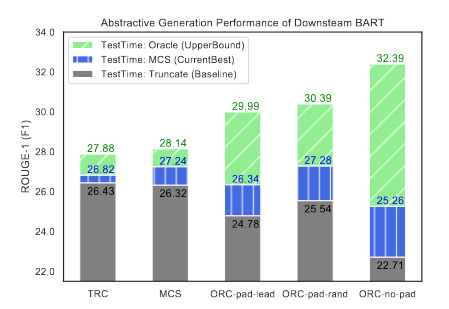
\includegraphics[width=10cm]{images/local_context2.png}
    %\centering
   % \caption{ The impact of training-time content selection methods on BART(1k) performance. Image credits: \citet{gales}}
    %\label{gales_fig2}
%\end{figure}

\citet{gales} seek to create a model involving heavy use of model-based feature selection combined with a conventional, transformer-based abstractive model. 

Before training, the input data is passed through a content selection algorithm. This can either be an "oracle" (referred to as "ORC" in the paper), which selects sentences based on the ground-truth (the ROUGE score of the selected input vs its abstract) or a pre-trained hierarchical, extractive model (referred to as "Multitask Content Selection" (MCS)). This approach is similar to the approached used by \cite{liu} in Section \ref{ssec::ClassificationSolutions}, although in this case the hierarchical approach did \textit{not} modify the base model, only acting as input pre-processing.

The "ORC" selection keeps an average of 21.3\% of sentences, drastically reducing the input's size and leads to 56\% of the input documents being shorter than the typical BART input span of 1024. There are three variants of the ORC selection method, including $ORC_{no-pad}$ which is deemed so aggressive as to inhibit training, $ORC_{pad-lead}$ which attempts to keep the sentence order and $ORC_{pad-rand}$ which pads missing sentences with random sentences from the input. Empirically it is shown that $ORC_{pad-rand}$ leads to the greatest performance yields.

The MCS model is a hierarchical encoder-decoder model with an attention mechanism built using RNNs (since their memory requirements scale linearly with the input size), a classification layer on top. 

Similar to the method used in \citet{lapata_bert}, the MCS model is simultaneously trained on an abstractive summarization task ($L_{seq2seq}$), in order to utilize the task-specific transfer learning property previously mentioned. The model is then also trained on the extractive summarization task ($L_{label}$). The training task is defined as follows:

\begin{equation}
    L_{seq2seq} = - \sum^{M}_{m=1} logP(y_m | y _{<m}, X)
\end{equation}

\begin{equation}
    L_{label} = - \sum^{N_1}_{i=1}(z_i log\hat{z}_i + (1-z_i) log(1-\hat{z}_i))
\end{equation}

\begin{equation}
    \hat{z}_i = sigmoid(\mathbf{W}^T_{cls} \mathbf{h}_i + \mathbf{b}_{cls}) 
\end{equation}
where $\mathbf{h}_i$ is the sentence-level encoder output associated with sentence $i$ and $\mathbf{W}_{cls}, \mathbf{b}_{cls}$ are the parameters of the classification layer.

\begin{equation}
    L_{MCS} = \gamma L_{label} + (1-\gamma)L_{seq2seq}
\end{equation}
where $\gamma$ is a hyperparameter.

During inference the sentences are scored as follows:
\begin{equation}
    score_{i, label} = \hat{z}_i, score_{i, seq2seq} = \sum^{M}_{m=1} \mathbf{a}^s_{m,i}
\end{equation}
where $\mathbf{a}^s_{m,i}$ is the sentence-level attention weight at decoder step $m$ over input sentence $i$.

The model seems to struggle when limited to selecting a few sentences, and as such selects as many sentences as can fit inside the BART model. 

%A comparison of the training-time results of content selection can be found in Figure \ref{gales_fig2}. 

The abstractive model being fed the input is a modified version of the BART \cite{bart} model called LoBART. LoBART was inspired by the Longformer \cite{longformer} and Sparse Transformer \cite{child} models. It features 12 BERT layers for the Encoder and the Decoder respectively. The Encoder is pre-trained on the standard BART-Large-CNN embeddings. In fact, one of the defining reasons for the decision to use BART and not a Sparse Transformer, is the unavailability of such pre-trained embeddings. 

The defining difference of LoBART is that unlike the models above, it utilizes only local and not global attention. This allows the model to drop its memory requirements significantly, at the cost of missing context over large spans of text. The researchers use a window of $W=700$ tokens, which is calculated as $2 \times D$ where $D$ is the empirical average attention distance of $D \in [250, 350]$ tokens for an attention mechanism with uniform weights, attending to a distance of $1024$. Even with this compromise, important context may still be missed, especially in long documents. As such the model relies on the pre-processing feature selection models mentioned above in order to significantly increase its context span. 

During inference, the test data is first processed by the MCS model since ORC "cheats" by utilizing the input labels, and it can therefore not be used on the test data. Then the input is fed to the LoBART model. This approach leads to significant improvements in memory and processing time, as well as state-of-the art results in the arXiv, PubMed and Spotify Podcast datasets. %A diagram showing the training and inference pipeline can be found in Figure \ref{gales_fig1}.


\paragraph{Combining Top-Down and Bottom-Up Inference} We close with a generic training and inference framework which aims to share global and local context between the token representations.

%\begin{figure}
    %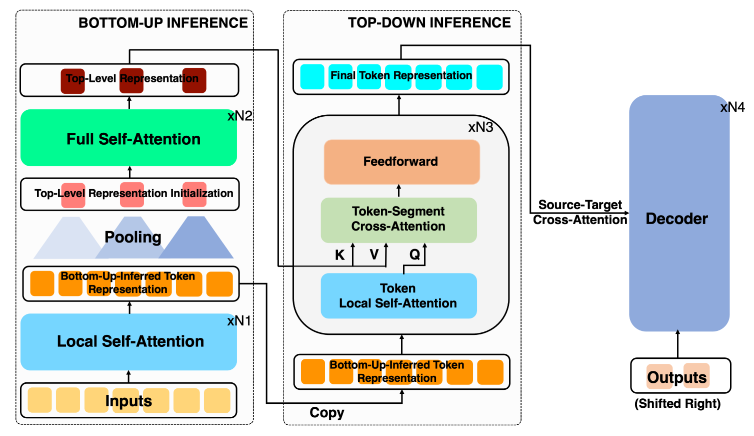
\includegraphics[width=10cm]{images/pan.png}
    %\centering
    %\caption{An overview of the top-down transformer. The bottom-up inference is achieved with local self-attention (N1 layers) as shown in the left panel. To initialize the top-level representations, we pool bottom-up-inferred token representations with either equal weights or adaptive weights. Top-level representations are then updated with full self-attention (N2 layers) to capture global context. They are then used to update bottom-up-inferred token representations, accounting for the top-down update for token representations, as shown in the middle panel. The final token representations are attended by the decoder to generate a summary.  Image credits: \citet{pan_bottom}}
    %\label{fig::pan}
%\end{figure}

\citet{pan_bottom} propose a new methodology where information flows from the tokens to the document embedding (bottom-up) and from the document embedding to the tokens (top-down). This is the result of two key observations on Sparse Transformers:

\begin{itemize}
    \item The quadratic cost of Transformers forces models to discard information about long-range context by using local self-attention.
    \item The models can use full self-attention on top-level representations (e.g paragraph embeddings).
\end{itemize}

The problem thus is that in a purely bottom-up framework (such as most Sparse Attention Transformers) the tokens do not have access to aggregated information form the entire document, while the top-level representation (document embedding) does not have access to the details provided by the tokens.

The researchers thus propose that the top-level representation be fed back to the tokens through all intermediate layers. These intermediate layers are not strictly defined and may be defined semantically (e.g word, sentence, paragraph, chapter, document) or mathematically (e.g sections with respective sizes $\frac{\text{doc\_length}}{256}, \frac{\text{doc\_length}}{4}, \text{doc\_length}$). The lower-level layers are assigned local self-attention because of their numbers, while higher-level layers can afford to be assigned full self-attention.

Specifically, the lower-level representations are updated in three transformations:
\begin{enumerate}
    \item Token self-attention
    \item Token-segment cross-attention
    \item Feed-forward
\end{enumerate}

%The full top-down transformer is shown in Figure \ref{fig::pan}.

The researchers use a single top layer, and define the layers as fixed-sized segments in order to avoid complicated implementation featuring varying-length input sizes. They also try using Average Pooling (AvgPool), Adaptive-weight Pooling (AdaPool) and Oracle Pooling (OracleAdaPool) functions in-between layers. Their model achieved competitive results in small-to-medium datasets such as CNN/Daily Mail, state-of-the-art results in Long Document datasets such as arXiv and PubMed, and competitive performance in the BookSum \cite{poland} and SummScreen \cite{summset} datasets, with a fraction of the cost and training data of the SOTA models.

The proposed method is model-agnostic and can be used for any Seq2Seq model. In fact, a version of this method was used in the Hi-Transformer \citet{qi} (Section \ref{sssec: HierBERT}). This fact will hopefully make the method applicable to general Transformer frameworks and other NLP tasks such as Document Classification.


\section{Sentiment Analysis / Opinion Mining}
\label{sec::Sentiment}

\textbf{Opinion mining (OM)} or \textbf{Sentiment Analysis (SA)} is a field of research that uses Natural Language Processing in order to get information from a text that helps in extracting ideas and opinions and presenting the information in an efficient way \cite{pakistan, sergio}. 

Sentiment analysis has witnessed remarkable commercial success due to its ability to unlock valuable insights from vast amounts of unstructured textual data. By leveraging natural language processing (NLP) techniques, sentiment analysis algorithms can effectively gauge the sentiment or emotion expressed in texts, such as social media posts, customer reviews, and online discussions. This invaluable tool has found significant applications across various commercial fields. In the realm of marketing and brand management, sentiment analysis helps companies monitor public opinion and identify customer satisfaction or dissatisfaction \cite{sa_example_1, sa_example_2, sa_example_3}. Sentiment analysis also finds utility in political analysis, where understanding public sentiment is crucial for informed decision-making \cite{sa_example_4, sa_example_5}. For a more in-depth review of Sentiment Analysis Applications, we recommend \citet{sa_applications}. However, SA has not been used extensively for large documents, since most commercial applications only need to deal with short tweets, posts and comments. 

Long document SA can be used for literary works, in order to process narrative hints. For example, it can be used in to determine characters' emotional states throughout the text, which can then help with Document Classification, as the emotions portrayed in eg. a book can help us figure out its genre. It can also be used for identifying key narrative points and sections and anticipated reader feelings as described in \citet{omori}. These observations however are almost purely theoretical at this point, since there appears to be no current research on literary analysis on whole books.


\subsection{Challenges}

Most of the techniques used in OM/SA use a bag of words known as "Sentiment Lexicon", which are words that are heavily weighed towards positive or negative emotions. For example words such as "good, bad, great, terrible etc." are likely candidates for a model's Sentiment Lexicon\cite{shelly}. This has been helpful for researchers on a baseline level but presents them with a few challenging problems such as:

\begin{enumerate}
    \item Sarcasm: As with Document Classification, sarcasm and non-literal use of such words creates a problem where the models falsely label a sentence because of these words appearing in it, without understanding their usage.
    
    \item Lack of appropriate Sentiment Lexicon candidates: In texts that use complicated vocabulary we often find ourselves lacking "simple", key words included in most Lexicons and thus most systems struggle to classify the emotions behind these sentences accurately.

    \item Polysemy: The issue with document-level sentiment classification is the challenge in encoding semantic and syntactic relations between sentences to the semantic meaning of the document. For example, the words "contrast" and "cause" can completely flip the class of a document (see Section \ref{ssec::ClassificationChallenges}: Polysemy). 
\end{enumerate}

Additionally, long document SA faces challenges common to the other NLP tasks, outlined in Sections \ref{ssec::ClassificationChallenges} \ref{ssec::SummarizationChallenges} such as demanding computational costs, long-spanning dependencies and sentiment variation across different sections or paragraphs.
	
\subsection{Solutions}

\subsubsection{Early Work}

One of the earliest studies on Sentiment Analysis \cite{pang2} uses simple machine learning algorithms like Naive Bayes, Maximum entropy and SVMs in a dataset of movie reviews in order to predict the reviewers' sentiments. Through studies like this, the aforementioned "sentiment lexicon" grew as researchers had more and more information about the frequency of certain terms used by people in a certain emotional state.  

The same researchers two years later \cite{pang} used the same machine learning methods to explore the question of "Is x sentence objective or subjective?", again using movie reviews as the dataset for both training, validation and testing. Using these simple models, researchers were able to achieve upwards of 87\% accuracy, which at the time, was a huge improvement.  

Another problem that was explored early on was sarcasm detection. One of the earliest works on sarcasm detection was \citet{stacey} in 2003, which introduced the "6-tuple representation", and it is considered to be a very important milestone in sarcasm identification in linguistics. They defined sarcasm as a sentence consisting of 6-tuples where: $S$= Speaker, $H$= Listener, $C$= Content, $u$= Utterance, $p$= Literal proposition, $p’$= Intended proposition.

In their attempt to solve the problem of sarcasm detection, most researchers have started using social media sites such as Twitter to train their models \cite{dmitry}, paying special attention to the amount of hyperboles used in sarcastic sentences to aid them. This is done because of the vast amount of easily accessible data and the syntax and form of tweets (short sentences). A 2017 study on sarcasm detection \cite{shelly} using Deep Convolutional Neural Networks was able to reach upwards of 90\% accuracy.


\subsubsection{Use of hybrid architecture models} 
 
Early Sentiment Analysis research was mostly done using small texts such as tweets, since datasets for long documents were not that prevalent and the machine learning architectures at the time were not as developed. However, as time passed we started seeing more and more interest in longer text Sentiment Analysis. For example, \citet{tang} create a model which uses a hybrid CNN and LSTM\cite{LSTM} architecture to classify long, document-level ratings on the IMDB dataset \cite{diao} and the restaurant review datasets from the 2013, 2014 and 2015 Yelp Dataset, achieving state-of-the-art results.  

In order to solve the issues of Polysemy (see Challenges: Polysemy) They exploit the "principle of compostitionality" \cite{francis}, which states that the meaning of a body of text (a sentence, a paragraph or a document) depends on the meanings of its constituents, by using a CNN or LSTM to produce sentence embeddings. These sentence embeddings are later used by a gated recurrent neural network (a variation of the LSTM architecture) which encode their relations and semantics in document representations. The gated units can be viewed as a LSTM whose output gate is always on, since they deem necessary that all available semantic information in the sentences be used in the document representation.

Furthermore, the document representations are used as features and classified. Specifically, they are turned into float-valued vectors by a linear layer, and fed to a softmax layer. Depending on the architecture of the model, the output of the softmax layer can either be a character's opinion or sentiment.

One of the most recent Sentiment Analysis papers which does not use transformers\cite{morocco} uses a similar architecture, combining CNNs and BiLSTM, the latter meaning Bi-Directional LSTM. The dataset they created and used was one of newspaper articles, each containing an average of 4000 words and they used Doc2Vec\cite{doc2vec} for the generation of document embeddings. The researchers then tested multiple architectures such as pure CNNs, LSTM, CNNs and LSTM, CNNs and BiLSTM and decided on the latter one as its results surpassed the others. Another recent research paper on sentiment analysis\cite{1453} uses GRNNs\cite{GRNN}, which are a variation of LSTM with a reset gate $r_t$, an update state $z_t$ and manages to achieve state-of-the-art results.

\subsubsection{BERT-based Models and key entity detection} 

Most modern day models make use of transformers, with BERT and its variations being very commonly used for Sentiment Analysis. \citet{toutanova} found that BERT models outperformed other state-of-the-art NLP models on a variety of Sentiment Analysis benchmarks. They achieved this by fine-tuning the BERT model on the specific task of Sentiment Analysis, rather than using it as a general-purpose NLP model.

\citet{xinzhao} goes into further detail on Sentiment Analysis using multiple BERT-based models as well as some more outdated ones to perform SA on financial texts, suggesting a model based on RoBERTa (Robustly Optimized BERT Pretraining Approach) as the one with the best results. It is plausible that the conclusions drawn in the paper will help develop models that analyse long texts in the near future.



\section{Long Document Datasets}
\label{sec::Datasets}

Applying NLP methods to large texts, and especially literature, is still a research area that largely remains unexplored. Compared to processing small texts such as quotes and tweets, the amount of data and research that has gone into it still remains fairly limited. However there has always been an interest in understanding and processing large texts. As early as 2007, with the release of the first version of the OntoNotes dataset\cite{ontonotes}, researchers accessed the ability to train models using data from some large texts. Many other general-use NLP datasets include large texts, such as the OPUS dataset that also allows for bilingual model training\cite{tiedemann}, which in turn makes tasks such as generating subtitles significantly easier.  

The earliest large-document dataset which contains only literature texts is the Columbia Quoted Speech Attribution corpus \cite{elson}. This dataset contains annotated English literature texts from the 19th and 20th centuries while putting emphasis into quoted speech, as it was made to solve problems such quotation extraction and speaker identification, however its data can still be utilised for other purposes, such as the ones described in this paper. 

Additionally, a really interesting modern dataset for literature texts is LitBank\cite{bamman}, a dataset of 100 English literature works that fully includes word annotations and co reference relations between words that belong in different groups. Models trained using this dataset seem to significantly outperform ones trained using older datasets such as OntoNotes, since this one is particularly focused on English Literature texts, compared to its more general counterparts.  

Another interesting dataset is the CSL\cite{li} dataset, developed in 2022 which includes a plethora of Chinese scientific literature books. Models similar to BERT that were trained on this dataset achieved really high accuracy in tasks such as Document Classification for a language as complicated as Mandarin which is even more impressive considering the train and test data are specifically scientific literature, which contains a larger variety of words compared to standard literature. 

Concerning Document Summarization, the traditional dataset used was the CNN/DailyMail dataset \cite{nallapati2}, featuring over 330k articles and their respective highlights, as written by journalists at CNN and the Daily Mail. Each article has a mean $781$ input tokens, and $56$ summary (target) tokens. While the dataset is certainly large, and shipped with developed and convenient APIs \cite{tf_cnn_dailymail, kaggle_cnn_dailymail, hugging_face_cnn_dailymail} because of its age and prominence, the individual articles may not be long enough for models specializing in long Document Summarization. This has not stopped it from being featured as a benchmark for long-document models to also demonstrate their efficiency in short-to-medium length documents however\cite{big_bird} .

Because of this concern, two datasets have rose into prominence the last few years in the field of Document Summarization, those being the arXiv \cite{clement} \cite{gong} and PubMed \cite{sumpubmed} \cite{franck} datasets. Their rise can be attributed to the huge number of documents, significant document length (since they both feature research articles), and user-curated summarizations in the form of abstracts. Their success as datasets is evident from their inclusions in many popular machine learning libraries \cite{tf_datasets} \cite{kaggle_arxiv} \cite{hugging_face_arxiv} \cite{hugging_face_pubmed} and their use as benchmarks for comparing state-of-the-art summarization models. 

Recently, two more challenging datasets have been released, those being the BookSum \cite{poland} and SummScreen \cite{summset} datasets. BookSum covers books from multiple domains in literature, including stories, novels and plays. SummScreen includes movie plots from their scripts. Both of these datasets require combining plot events from implicit subplots, some progressing in parallel, forcing models to rely on extremely long context spans and dependencies.

Domain specific datasets are crucial for domain-specific models, either to be used for training or re-training general pre-trained NLP models in order to increase their accuracy in that particular domain \cite{dai}. Below is a brief list of such datasets featuring primarily long documents and used in Document Classification and/or Document Summarization tasks;

\begin{itemize}
    \item \textbf{LexGLUE} \cite{glue_gunner}, a benchmark dataset containing a collection of smaller datasets of legal cases.
    
    \item \textbf{MIMIC-III} \cite{mimic} ('Medical Information Mart for Intensive Care'), which contains Intensive Care Unit (ICU) discharge summaries. This dataset has the benefit of being annotated with labels following the ICD-9 (The International Classification of Diseases, Ninth Revision) hierarchy.

    \item \textbf{ECtHR-LJP} \cite{ion3} containing approximately 11,000 cases from the European Court of Human Rights, where each case is mapped to the paragraphs of ECHR which were allegedly violated.

    \item \textbf{ECtHR-ARG} \cite{habernal} which similarly to \cite{ion3} contains cases from the European Court of Human Rights, but which also provides a list of \textit{argumentative paragraphs} from the analysis of the case. Note that this dataset only contains about 300 cases.

    \item \textbf{ContractNLI} \cite{koreeda} a dataset for document-level Natural Language Inference (NLI) for contracts, where each data point is annotated with multiple labels indicating whether the content agrees with, contradicts or doesn't mention any of many hypotheses.

    \item \textbf{20 Newsgroup} \cite{20groups} a dataset containing approximately 20,000 newsgroup documents partitioned evenly 20 different newsgroups. This dataset provides a great amount and variety of data, but its articles tend to be significantly shorter than dedicated long-document datasets.

    \item \textbf{Hyperpartisan News Detection} \cite{hyperpartisan} which contains documents for political standpoint classification. This dataset contains both long and short articles, and thus a split must be performed based on the data's length for long-document NLP tasks.
\end{itemize}


    \section{Summary}
    \label{sec::Summary}
    We summarize the problems, solutions and relevant research mentioned in this paper in Table \ref{tab::text_class_table} for Document Classification and Table \ref{tab::text_sum_table} for Document Summarization.

    \begin{table}[H]
        \scriptsize
        \begin{tabular}
             { |p{3cm}|p{3cm}|p{9cm}|  }
             \hline
             \textbf{Method} & \textbf{Addressed Problems} & \textbf{Details}\\
            \hline
             \multicolumn{3}{|c|}{Metrics \& Preprocessing} \\
             \hline
             Measuring Multi-class Label Accuracy \cite{sicong}  & Multiple / Varying Count of Labels & By using a multi-label output metric any classifier's accuracy can be measured effectively both for multiple classification and a variable count of labels for each different document.\\
             \hline
             Feature Pruning \cite{sicong, worsham}& Dataset Size \break \break Computational Cost & Ruthless pruning and careful selection / sampling can significantly cut down on the computational costs of huge datasets and very long documents. On the other hand, even words traditionally considered semantically useless can be significant for a model to understand subtle grammatical and syntactical rules.\\
             \hline

             \multicolumn{3}{|c|}{Sparse Transformers} \\
             \hline
             
              Sparse Transformers \cite{sparse_attention} & $O(n^2)$ Transformer Cost & By utilizing a sparse attention mechanism, and with various mathematical optimizations, a standard Transformer model can become viable at parsing entire long-document inputs.\\
            \hline
             Dilated Sliding Window \cite{longformer} & $O(n^2)$ Transformer Cost \break\break Context Fragmentation & Using a dilated sliding window technique, while also allowing a limited number of global tokens, the modified Transformer model becomes capable at successfully parsing ever-increasing-length documents, while keeping track of local context.\\
             \hline
             Sliding Window + Random Selection + Global Attention\cite{big_bird} & $O(n^2)$ Transformer Cost \break\break Context Fragmentation & Combining Longformer's sliding window, block attention scheme, and random token selection can encapsulate local and global context more efficiently while keeping computational costs low. \\
             \hline

             \multicolumn{3}{|c|}{Hierarchical Transformers} \\
             \hline
             Hierarchical Transformers with traditional networks \cite{ion_han, zichao, khandve, use} & Transformer Input Limit & Instead of using Transformer models for the entire document, they can be used to produce segment embeddings, which are then combined by traditional networks (HAN, LSTM, CNN).\\
             \hline
             Hierarchical Transformers with BERT \cite{qi} &
             Global Context \break\break Context Fragmentation & BERT models can be used to produce sentence embeddings, then document embeddings which can be fed back to new, context-aware sentence embeddings iteratively.\\
             \hline
             Hierarchical-Sparse Transformers \cite{liu} & $O(n^2)$ Transformer Cost \break\break Local/Global Context issues \break\break Position Overfitting & By using a hierarchical architecture embedded in a Sparse Transformer, and by providing a new loss function rewarding token position invariance, the model is able to effectively handle global context and become invariant to small modifications of the input text.\\
             \hline

             \multicolumn{3}{|c|}{Recurrent Transformers} \\
             \hline
             Recurrent Transformers \cite{dai} & $O(n^2)$ Transformer Cost \break\break Context Fragmentation \break\break Global Context & By keeping the context of previously inputted segments in hidden states and by utilizing relative positional embeddings, the transformer model can not only decrease its asymptotic complexity, but also multiply its size during inference irrespective of its size during training. \\
             \hline
             Skimming Recurrent Transformers \cite{dai-etal-2019-transformer} & $O(n^2)$ Transformer Cost \break\break Context Fragmentation \break\break Global context \break\break Forward context & Forward and global context of greater quality can be obtained by passing through the input text twice, once by peeking small text segments (skimming phase), and then by performing a full pass (retrospective phase), fully utilizing the recurrence mechanism. \\
             \hline
        \end{tabular}
        \caption{Problems and Solutions for Document Classification for long documents}
        \label{tab::text_class_table}
    \end{table}

    
    \begin{table}[H]
        \scriptsize
        \begin{tabular}
             { |p{3cm}|p{3cm}|p{9cm}|  }
             \hline
             \textbf{Method} & \textbf{Addressed Problems} & \textbf{Details}\\
            \hline
            
             \multicolumn{3}{|c|}{Extractive Document Summarization} \\
             \hline
             Building Summaries Using Hierarchies \cite{lapata, nallapati, xiao} & DNN use for summarization  \break\break Document Structure under-utilization & Older models attempt to explicitly incorporate context and hierarchical elements to the features used by CNN, RNN and LSTM extractive models. \\
             \hline
             BERTSUM-Ext \cite{nallapati2} & Poor traditional DNN performance\break\break Weaknesses in Sentence Embeddings & By using BERT as encoder-only and attaching stacked Transformer layers, BERT's expressive power can be used to produce accurate extractive summaries.\\  
             \hline
             HiStruct+ \cite{histruct} & Segment/Document Context Loss\break\break Under-utilization of Document Structure & By encoding the hierarchical and topical structure of a document, the Transformer model can leverage mor information rigid and hierarchical documents such as research articles.\\
             \hline
             HEGEL \cite{hegel} & Under-utilization of Document Structure\break\break $O(n^2)$ Transformer Cost\break\break Long-span-dependencies & Encoding each document as a hypergraph under multiple different views leads to the model being exceptionally adept at summarizing very long and rigidly hierarchical documents.\\
             \hline

             \multicolumn{3}{|c|}{Abstractive Document Summarization} \\
             \hline
             Pointer Generated Networks \cite{abigail} & Word Repetition\break\break Vocabulary Limitations\break\break  Long Document Computational Cost & By allowing the network to choose whether to copy a word from the source text or produce its own, the model can benefit from a significantly expanded vocabulary, reduce computation costs by keeping a smaller vocabulary and mostly bypass the word repetition problem found in many extractive summarization models. \\
             \hline
             Sparse Attention Transformers \cite{longformer, big_bird} & $O(n^2)$ Transformer Cost \break\break  Vocabulary Limitations & By using a modified sparse transformer as the encoder, the model can leverage the expressive power of transformer models on long documents. \\
             \hline
             Local Attention and Content Selection \cite{gales} & $O(n^2)$ Transformer Cost  \break\break Long Document Computational Cost & Pre-trained models can be used for content selection in order for a Sparse Attention model to be fed only useful data, both in training and inference.\\ 
             \hline
        \end{tabular}
        \caption{Problems and Solutions for Document Summarization for long documents}
        \label{tab::text_sum_table}
    \end{table}

 
	\section{Conclusion}
    \label{sec::Conclusions}
	
	Analyzing long documents currently presents a daunting challenge, even with the recent breakthroughs in NLP research. While traditional machine learning and statistical methods provide some functionality on these tasks, they ultimately prove less adaptable and less accurate than neural network models. However, not only do neural networks need to face traditional issues such as the curse of dimensionality, they must also overcome limited datasets, prohibitively large inputs and difficult writing formats such as ones used in literary works.  
 
    Most major problems are common to many long NLP tasks and tend to require similar solutions, such as limiting the model's vocabulary, modifying existing Transformer architectures and artificially augmenting the training datasets. There are also task-specific solutions, such as using model/oracle-based feature selection and specialized GNNs to capture long-spanning context in Automatic Document Summarization tasks and passing over the input twice and using document-level representations to enrich and re-code sentence-level representations in Document Categorization tasks. While this survey focuses on only two of these tasks, it becomes apparent how attempts at solving task-specific problem can, and in some cases already have, propagated to solutions for generic long-document NLP challenges which impact all NLP tasks. It is however important to note that these solutions simply provide neural network models with useful trade-offs and are therefore not to be used universally. We also note the potential for research into Literary Sentiment Analysis, since the necessary theoretical background already exists, while the mentioned breakthroughs in long document NLP tasks have not been yet applied. 
    
    Long document NLP analysis is a field in its infancy and breakthroughs leading to large jumps in computational efficiency and accuracy are frequent. Since 2015 neural network models have evolved from being constrained to (sometimes artificially) small sized documents, to being able to effectively parse large articles and literary works. We are therefore confident that research will help bypass most of the current limitations. 
	
	
\bibliographystyle{elsarticle-num-names} 
\bibliography{refs}
\end{document}
\endinput